\documentclass{article}
\usepackage[utf8]{inputenc}
\usepackage[english]{babel}
\usepackage[square,numbers]{natbib}
\usepackage{graphicx}
\usepackage{color}
\usepackage{subcaption}
\usepackage[section]{placeins}
\usepackage{amsmath}
\usepackage{amsfonts}
\usepackage{listings}

\bibliographystyle{abbrvnat}
\newcommand{\js}[1]{{\color{red}{[#1]}}} 
\graphicspath{ {./graphics/} }
\def\mathit#1{\em #1}

\title{Generating and Smoothing Handwriting with Long Short-Term Memory Networks}
\author{Muchigi Kimari, Ikenna Nwagou, Edward Fry, Yumei Bennett,John Santerre}
\date{April 2021}

\begin{document}

\maketitle

\begin{abstract}
    This project explores the different neural network methods to generate synthetic handwriting text. The goal is to offer an AI tool that generates handwriting, while maintaining an individual's style, to people suffering with Dysgraphia. As part of this project, an application development framework is setup on GitHub, in such a way that others can continue to explore and improve the AI tool.
\end{abstract}

\section{Introduction}

Since there is no common handwriting style, it is challenging to develop a tool that generates and smooths handwriting. However, the potential future application and rewards for helping people with Dysgraphia, on the hand, make this challenge worthwhile. Dysgraphia impacts a person’s ability to learn in many ways. One example of Dysgraphia’s effect on learning involves issues with fine motor skills. When a person develops an idea, or learns a new concept the best memorization technique is to repeatedly write the concept or idea on a piece of paper \cite{Dysgraphia_intro}. However, due to fine motor deficiency, people with Dysgraphia find writing simple text difficult, impeding their ability to memorize information.

Due to the nonlinear nature of Neural Networks, the possibilities for solving complex non linear problems are endless. Radiology can now keep up with image processing thanks to Neural Networks. Self driving cars can now map road marks to increase safety \cite{Radiology}. This research paper focuses on applying Neural Networks to recognize and smooth handwriting in order to assist people with Dysgraphia.

The application of Neural Networks has many techniques, but for this research papers the focus is on Long Short-Term Memory networks. LSTM models are good for solving handwriting recognition problems because they have the ability to memorize different styles and come up with a probabilistic and standard style of handwriting \cite{LSTM_Style}.

The goal of this project is to inspire and broaden the research on Dysgraphia and its effect on handwriting \cite{Paper_Intro2}.



% One page on why this is interesting problem
\section{Background}
Text recognition and generation has a long history, dating back before Neural Networks became a science research field. The telegraph, invented in the early 1910s, is regarded as first text recognition application. Since its inception, the telegraph has helped the blind to read and has made it possible to deliver short messages without expensive telephone calls\cite{previous-work-33}. Technology is always advancing looking for ways to increase accuracy and efficiency. Today, applications like scan to digital documents, text to speech audio books, tablet note taking, and smart phone language translation are not only widely available, but also relied on in our daily life and work\cite{previous-work-24}. 

In recent years, Neural Network development has fueled the advancement of text recognition and generation. There are two main categories of competing technologies in this area. The Optical Character Recognition (OCR) is the most popular method. It processes the printed or handwritten text as an image file, in pixel format, utilizing the neural network's mega data processing power to train the model. This method is referred to as the offline method\cite{previous-work-23}. The second category is the pen stroke position method, where the application collects pen stroke positions as time series data. The advantage of the pen stroke position method is that its data size is significantly smaller compared to OCR, making it easier to work with. This method requires a device to collect pen position as the writer creates the text, and it is referred to as the online method. Figure~\ref{fig:YES} shows an example of online and offline text format.  

    \begin{figure}[hbt!]
        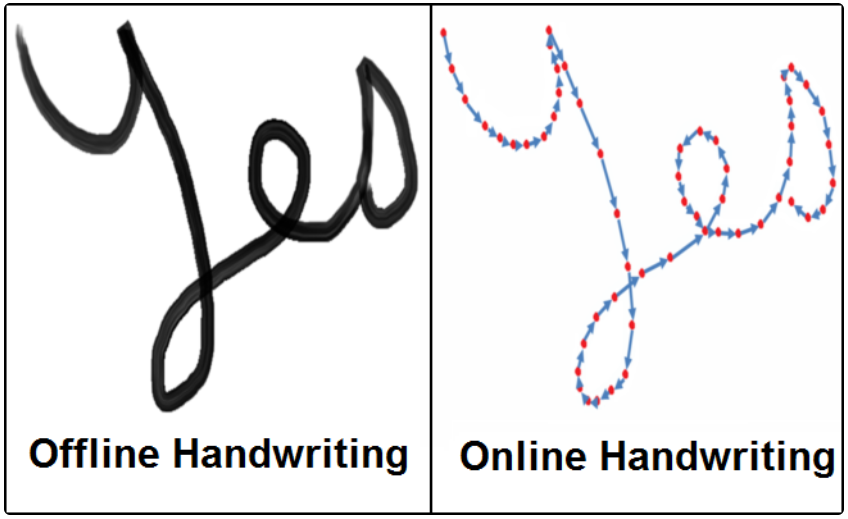
\includegraphics[width=12cm]{Capture.PNG}
        \centering
        \caption{Offline and Online Text Input\cite{Yes_online_offline_graph}}
        \label{fig:YES}
    \end{figure}

The primary research in the text recognition and generation areas are focused on commercially viable applications, such as medical form transcription, library archive digitization, enterprise data entry automation, and indexing document for search engines. Although just as important but less profitable, areas directed at helping the visually or vocally impaired, the autistic, or those suffering with a motor function disability like Dysgraphia are not as widely researched. This project focuses on establishing a base line application, to generate legible text with a handwriting style preference.   

\subsection{Dysgraphia}
Dysgraphia is a bio-neural system disorder that impacts the fine motor skills. Since Dysgraphia effects the hand and finger fine motor skills, the handwriting and artwork of a person with Dysgraphia may appear illegible or sloppy\cite{previous-work-31}. The severity of Dysgraphia varies from mild to severe. Mild symptoms may emerge as a dislike for handwriting due to the difficulties associated with fine motor skills. Severe symptoms may show as a visible hand tremor. In mild cases, Dysgraphia is often left misdiagnosed or mistaken for laziness or sloppiness. People with Dysgraphia often have other bio-neural system disorders like Dyslexia, Attention-deficit/hyperactivity disorder, or brain trauma\cite{Previous-work-32}. Although there is limited medical research on Dysgraphia to date, it is estimated that it affects two to 25 percent of the population. Dysgraphia was not  recognized as a neural disorder until 1993 by Hamstra-Bletz & Blote as a disturbance or difficulty in the production of written language that is related to the mechanics of writing\cite{Dysgraphia_recognized_date}. Prior to then, it was viewed as a symptom of Dyslexia.

Dysgraphia symptoms often appear when a child is starting to learn how to write and draw. Many schools do not recognize Dysgraphia in children. A child's lack of progress is often confused with not working hard enough, and at times, children with Dysgraphia are punished by assigning more home work, detention, or parental reports. Such oversights lead to low morale, depression, and withdrawal of these children\cite{previous-work-29}.

The handwriting of someone with Dysgraphia often appears illegible and cacographic. The figure~\ref{fig:amplitude}~\ref{fig:slant}~\ref{fig:spacing} shows a number of samples: letters appear more slanted then usual, are unevenly sized and spaced. 
    \begin{figure}[hbt!]
        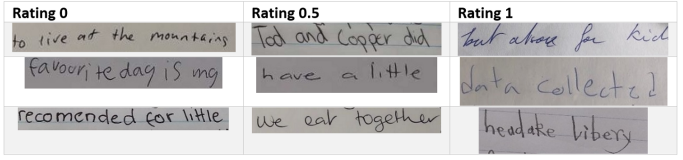
\includegraphics[width=12cm]{Capture.ampletude.PNG}
        \centering
        \caption{Dysgraphia Handwriting with Inconsistent Amplitude\cite{Dysgraphia_handwriting_graph}}
        \label{fig:amplitude}
    \end{figure}

    \begin{figure}[hbt!]
        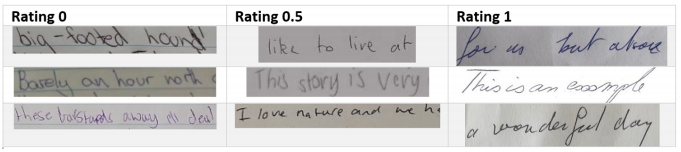
\includegraphics[width=12cm]{Capture.slant.PNG}
        \centering
        \caption{Dysgraphia Handwriting with Slant\cite{Dysgraphia_handwriting_graph}}
        \label{fig:slant}
    \end{figure}
    
     \begin{figure}[hbt!]
        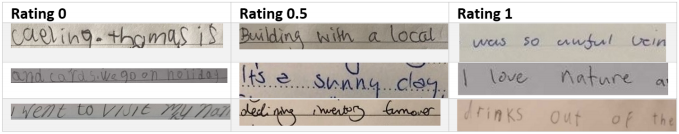
\includegraphics[width=12cm]{Capture.spacing.PNG}
        \centering
        \caption{Dysgraphia Handwriting with unusual spacing\cite{Dysgraphia_handwriting_graph}}
        \label{fig:spacing}
    \end{figure}


No cure for Dysgraphia exists, nor can it be outgrown. Dysgraphia in adults presents frustrating challenges every day. In offices, white boarding sessions are still a preferred way to collaborate, colleagues with Dysgraphia may struggle with these meetings. At home, a calendar is often full of handwritten notes, parents with Dysgraphia may ask others to write these notes.

With advancement in neural network methodology, success has been achieved in cursive hand writing recognition and generation\cite{previous-work-13}. This project's goal is to help children and adults with Dysgraphia by developing an AI tool that allows them to write in their preferred style, to empower them, and to encourage handwriting.



% https://totalability.ca/overcoming-dysgraphia/ child sample
% https://dystech.com.au/wp-content/uploads/2019/04/dyslexiaDysgraphia.pdf slant, amplitude, spacing


\subsection{Optical Character Recognition}
 The implementation of OCR systems in processing and digitization of paper documents is one example of previous work in handwriting recognition \cite{Previous-work-0}. In today's world documents come in many forms: printed, electronic, and written. The benefit of modern technology is the ability to create copies of written or printed materials, as well as archive these documents in a secure location such as the cloud. The limitations of modern technology become apparent when faced with handwritten, original, archaic documents. Previous work in handwriting recognition experimented with the application of OCR on different forms of documents. In the research, they discovered that processing and digitization of handwritten documents was problematic \cite{Previous-work-0}.  

With the utilization of neural networks, it is now possible to train with different styles of handwriting and build an application that can predict any written text. In addition to helping people with Dysgraphia, this work could be applied to recognizing old handwritten documents.
% what has been don on these problem and what is next
\section{Data}
\subsection{Structure}
The input data set is in the form of a set of XML files, each of which reflects the set of strokes belonging to a single sample of handwriting. The samples come from the IAM Online Database \cite{iam}. They were created by volunteers who wrote short phrases on an electronic device that captured the position of their pen in real time as they wrote. Each point captured has an $x$ and $y$ coordinate as well as a time stamp. This project will focus solely on the $x,y$ pairs. Here is a sample of one of the XML files:

    \begin{lstlisting}[language=XML]
        <WhiteboardCaptureSession>
          <WhiteboardDescription>
            <SensorLocation corner="top_left"/>
            <DiagonallyOppositeCoords x="6512" y="1376"/>
            <VerticallyOppositeCoords x="966" y="1376"/>
            <HorizontallyOppositeCoords x="6512" y="787"/>
          </WhiteboardDescription>
          <StrokeSet>
            <Stroke colour="black" start_time="769.05" end_time="769.64">
              <Point x="1073" y="1058" time="769.05"/>
              <Point x="1072" y="1085" time="769.07"/>
              ...
              <Point x="1215" y="1353" time="769.63"/>
              <Point x="1204" y="1330" time="769.64"/>
            </Stroke>
            <Stroke colour="black" start_time="769.70" end_time="769.90">
              <Point x="1176" y="1237" time="769.70"/>
              <Point x="1175" y="1233" time="769.72"/>
              ...
              <Point x="1010" y="1239" time="769.88"/>
              <Point x="1014" y="1243" time="769.90"/>
            </Stroke>
            ...
          </StrokeSet>
        </WhiteboardCaptureSession>
    \end{lstlisting}

After studying the data set and considering the needs of the training process (described below), a simple cascading series of one-to-many relationships emerges as the apparent data modeling choice. To reflect this structure in the application, a series of three objects is used. First, one \textit{Dataset} object represents the entire training data set and can be reused later to represent smoothing samples in a consistent way. Each \textit{Dataset} contains a list of stroke sets (\textit{StrokeSet}), where one stroke set represents the entirety of a single handwriting sample written by a volunteer, as shown in Figure~\ref{fig:example_handwriting_line}:

    \begin{figure}[hbt!]
        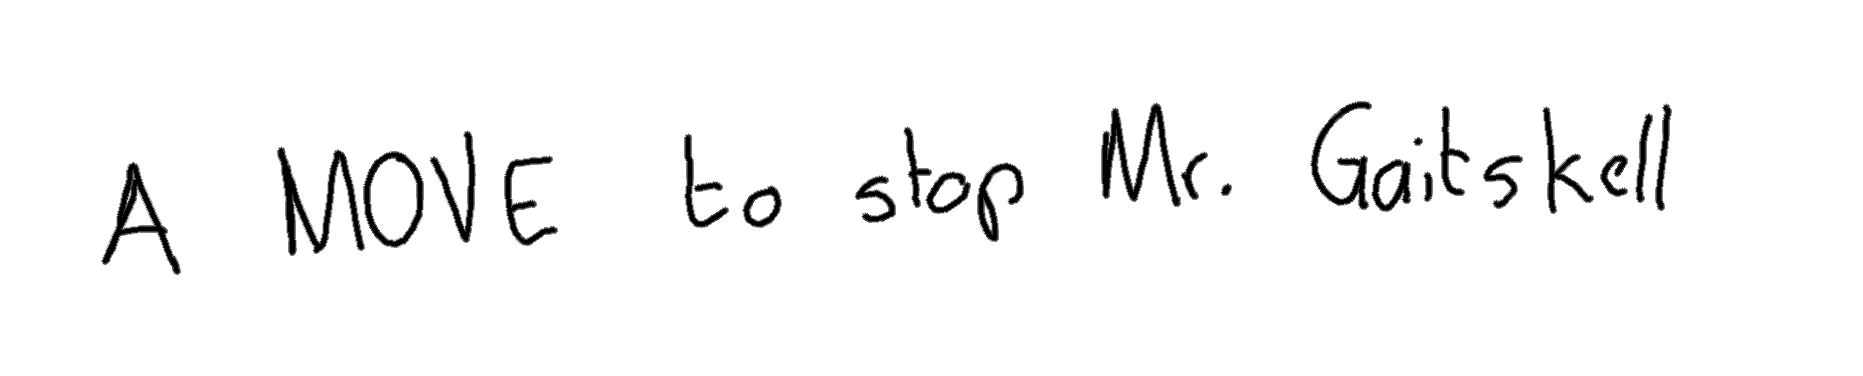
\includegraphics[width=12cm]{a01-000u-01}
        \centering
        \caption{Example of a training data point}
        \label{fig:example_handwriting_line}
    \end{figure}
    
Each stroke set then contains multiple strokes, stored as a list of \textit{Stroke} objects. A stroke is the set of points drawn between the time that the pen is set to the surface and lifted up again. Finally, each stroke contains a list of points. Each point is a fourth class (i.e. \textit{Point}) in this hierarchy even though, for practical and performance reasons, the points are simply stored as $x, y$ tuples in the stroke object. The entire conceptual structure of the application is expressed in this UML class diagram:

    \begin{figure}[hbt!]
        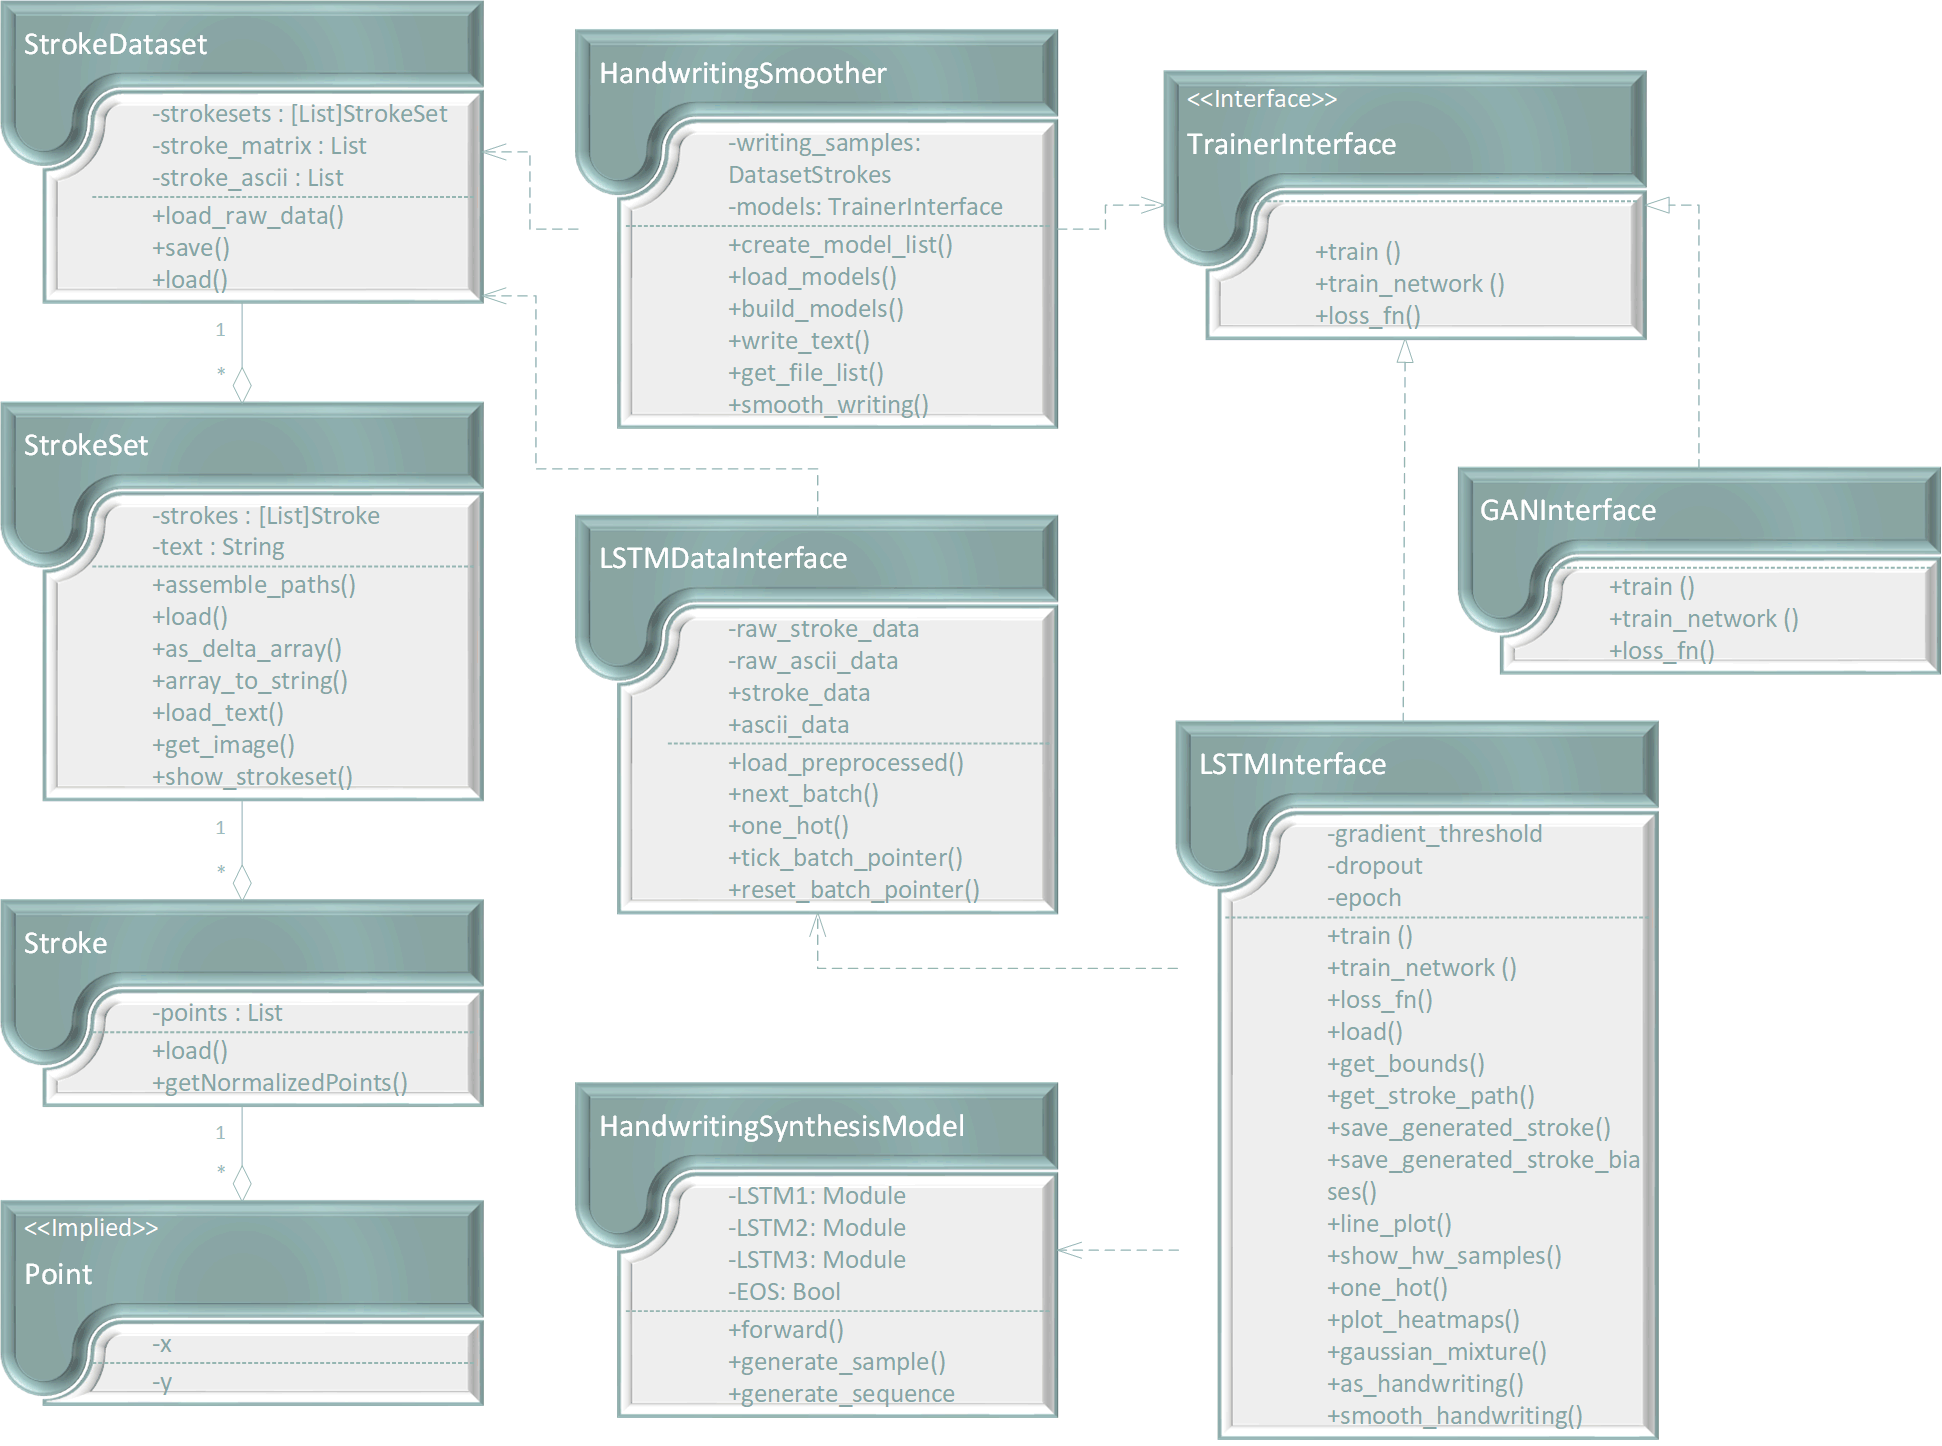
\includegraphics[width=10cm]{Classes}
        \centering
        \caption{UML class diagram for \emph{pywritesmooth}}
        \label{fig:uml}
    \end{figure}
    
Here is the complete picture of how the data in the input data set corresponds to its in-memory representation.

    \begin{figure}[hbt!]
        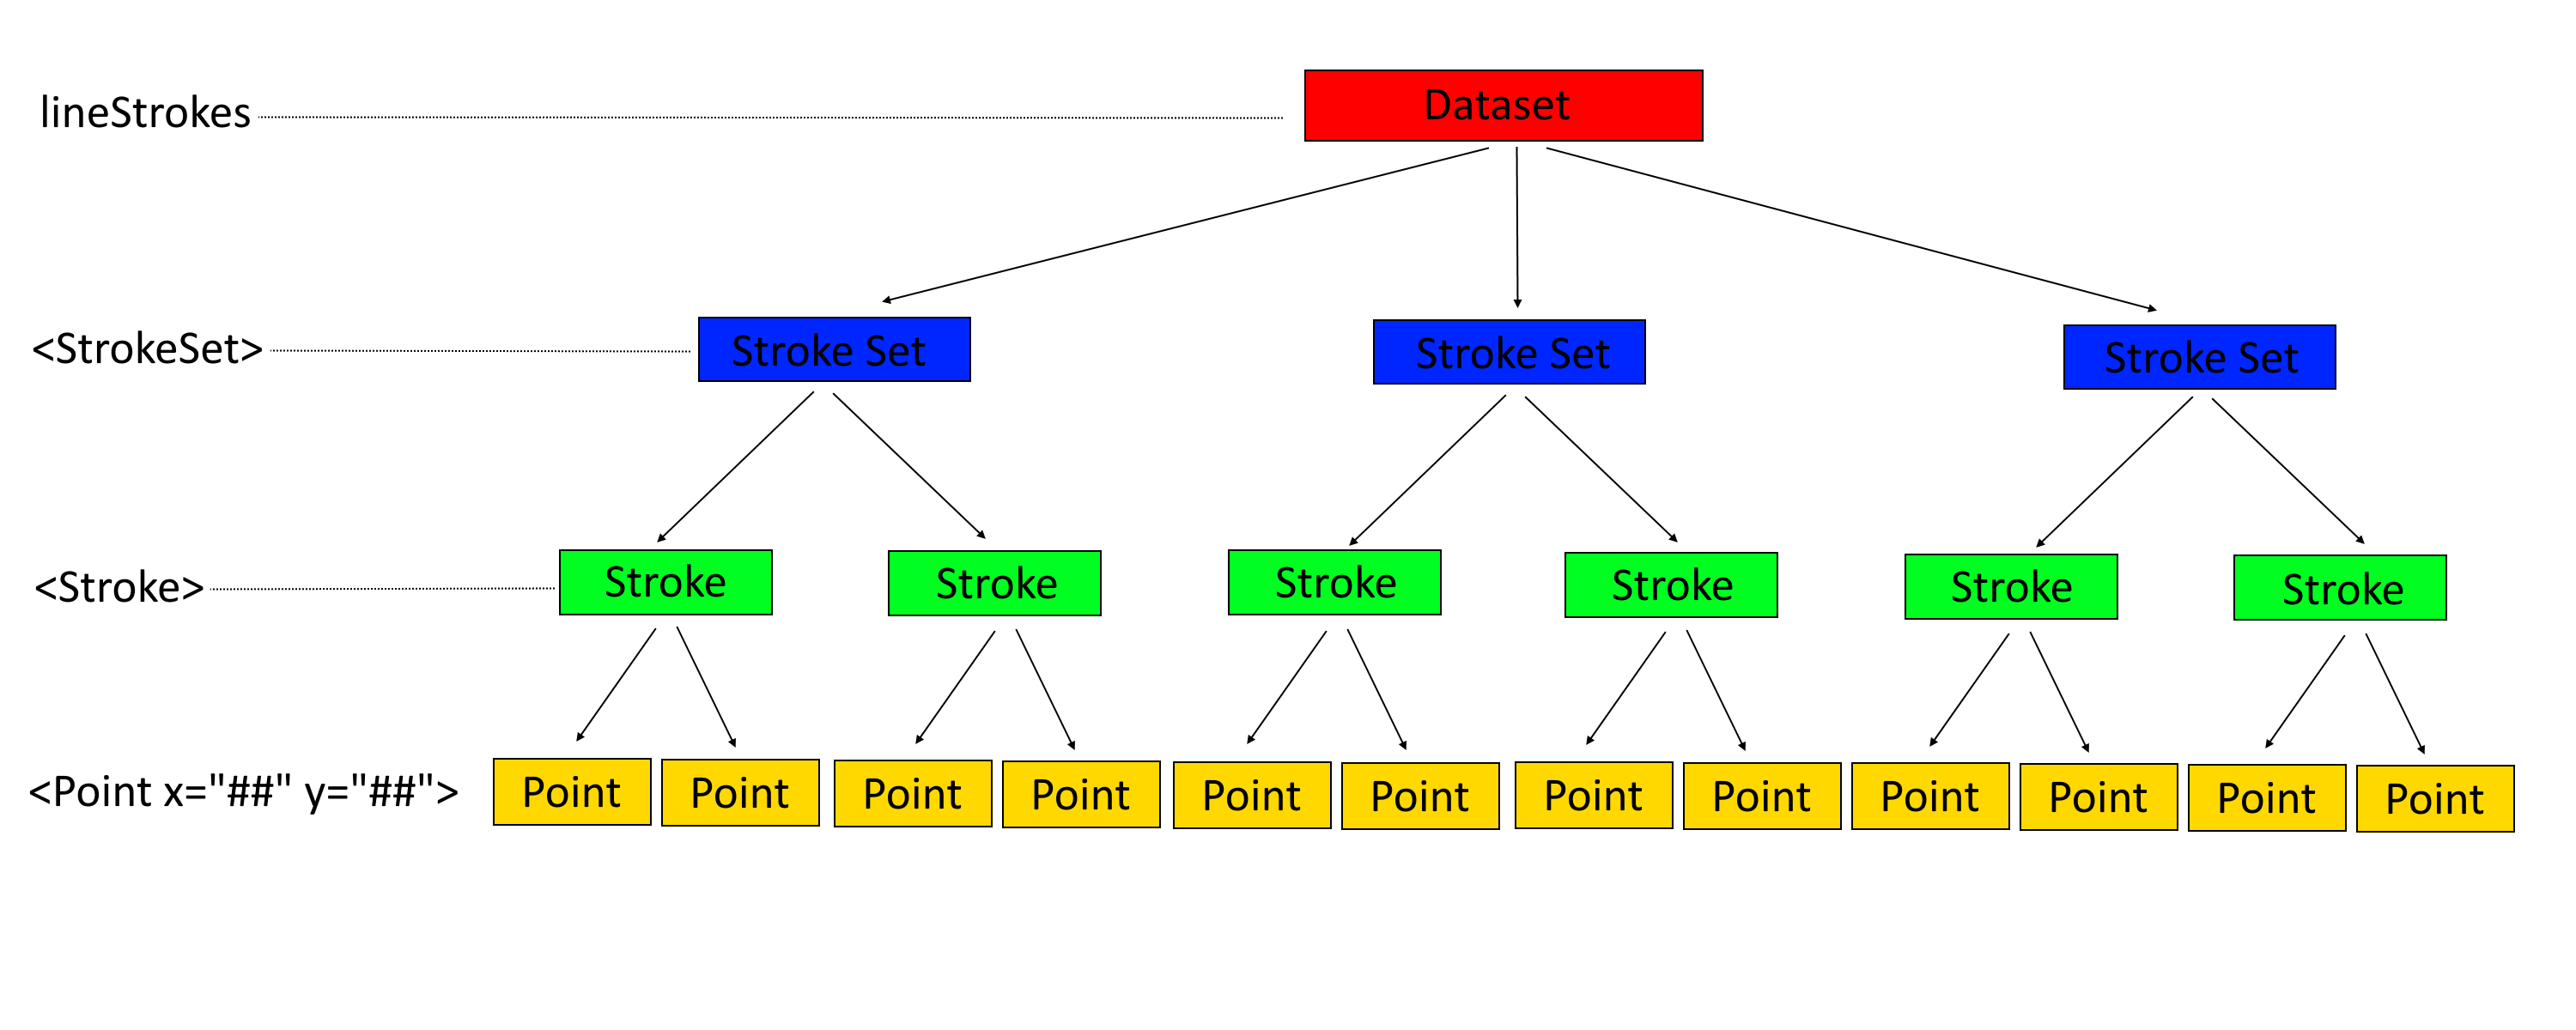
\includegraphics[width=12cm]{Dataset-Diagram}
        \centering
        \caption{Data mapping from XML to application classes}
        \label{fig:data-map}
    \end{figure}
    
\subsection{Model Training}
The second major functional area is training any models that are used. The specifics of training certain types are models are described later on. The application will support any number of models, which could be useful to compare the accuracy and performance of various approaches to the handwriting generation problem, for example.

In order to make use of this mechanism, simply implement the \textit{TrainerInterface} class, which requires methods to support training and a loss function along with methods to generate and smooth handwriting at a minimum. Models can also load themselves from a previously saved Pytorch model file, which saves time and computing power.

Once trained or loaded, the trained, ready-to-use models are available to the main program as a simple list of models. They can then be used individually or processed collectively using polymorphism. In this application, the only implemented model is currently \textit{LSTMTrainer}. \textit{GANTrainer} is provided as a placeholder for development testing purposes and still requires implementation. The \textit{HandwritingSynthesisModel} is a custom implementation of a Pytorch \textit{nn.Module} model and is used by the \textit{LSTMTrainer}.

\subsection{Handwriting Generation}
The final functional area of the program is that of handwriting generation. This takes two forms. In the first, a text string is provided (with a limit of 80 characters), and the trained model is then used to generate a sample of handwriting. Legibility can be controlled with the bias parameter, where higher values (up to 10 or so) will result in greater readability, and low values (to a minimum of 0) give greater variety at the expense of legibility. The resulting generated writing is saved in SVG format to the file name provided in the options.

The other function is to smooth handwriting. For this, a sample of handwriting needs to be provided using the appropriate option. The sample needs to be in the same format as the IAM data set that was used to train the model(s). Bias values control the legibility as described, and the generated handwriting is also saved as an SVG file. In addition, a plot of the sample in a variety of biases is saved for further study on the effects of bias to the generation.

\subsection{Application Workflows}
These three areas are combined below. The data set is read and processed into its internal object format. Any defined models are then trained. Finally, handwriting generation or smoothing is performed on the trained model(s).

\section{Methods}
Two approaches, generative adversarial network (GAN) and Long Short-Term Memory network (LSTM), were explored to generate and smooth handwriting; however, Long Short-Term Memory network (LSTM) provided the better outcome.

\subsection{GAN}
%what worked and what didn't
% data sets considered
GAN is a new convolutional neural network used for image processing. It is made up of two competing networks, which work together to generate a better model for prediction. The first network, the generator, takes an input and generates a false input, and then the second network, the discriminator, determines whether the input is true or false \cite{Dysgraphia_GAN}. The discriminator generates noise as its initial input, but as it learns, it generates better input data. This approach deals with processing handwritten images. Each image is split into words, then letters, and the final image input which is a letter image is used for learning and prediction. To achieve this, image extraction technologies such as Textract and OpenCV must be utilized. 

The metrics used for measuring the recognition accuracy are Precision and Recall. To be able to apply any of these performance metrics, the measure of the correctness of each detection needs to be established. For any given detection, a bounding box or a circle is placed on the object. The metric that measures the correctness of a given bounding box or circle is called the Intersection over Union (IoU). This is the ratio between the intersection and the union of the predicted box or circle and the grounding truth box \cite{Dysgraphia_IoU_evaluation}. Grounding truth box or circle is the correct box representation that would cover each letter. Twenty labeled image files from the data sample were used to measure the performance of each of the detection applications used, and then the mean precision and mean recall were recorded. Both the textract and openCV application had a mean precision of 0.9 and 0.8 respectively and a mean recall of 0.8 and 0.76 respectively. Textract performed better when compared with OpenCV because it is specifically designed to extract text and letters. Even though textract is able to recognize letters, there are instances where textract recognizes two letters as one and this poses a significant challenge.

\subsubsection{Training the Network}
The training mechanism was done outside of the main program of the application. In image processing, the individual pixels of an image are the data sample set, meaning a 28x28 black and white image would have 784 features. The input image was normalized from [0,255] to [0 to 1] before input into the neural network for training. Implementation of simple GAN and DCGAN (Deep Convolutional GAN) were types of GAN model used. The data sets used are EMNIST, MNIST, and UCI since they meet the requirements of individual printed numbers and letters in black and white. The models were configured to use 50 epochs and 100 batches. Both model struggled to generate a good results. This struggle could be that simple GAN and DCGAN are not complex enough to generate a better image. 

\subsubsection{Computational Considerations}
The models utilized the CUDA properties of pytorch which uses GPU. Using GPU helped speed up the training of the models.

\subsubsection{Visualizing the Training}
In the implementation of the training process, tensorboard which is a tensorflow's visualization toolkit was used to capture the image as model trained. This is crucial since GANs do not have a measurement metrics to measure the models performance. Capturing the images as it trained and comparing both the real images and the fake images shows how well the models are training. The goal is for the real image to be identical to the fake image so that they are indistinguishable by the human eye. The learning process for both models is illustrated in the figures below.

\begin{figure}[hbt!]
    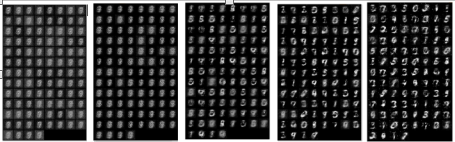
\includegraphics[width=12cm]{graphics/simpleGan.png}
    \centering
    \caption{Learning Progression for simple GAN}
    \label{fig:Simple GAN}
\end{figure}
    

 \begin{figure}[hbt!]
    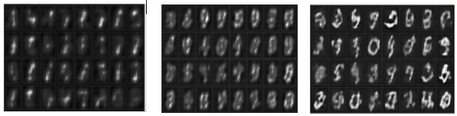
\includegraphics[width=12cm]{graphics/DCGAN.png}
    \centering
    \caption{Learning Progression for DCGAN}
    \label{fig:DCGAN}
\end{figure}   

    
\subsection{LSTM}
The work here is based largely on a paper by Alex Graves \cite{DBLP:journals/corr/Graves13}.  The reader should consider studying that paper first to maximize understanding of both LSTMs and handwriting generation before proceeding.  In addition, portions of the implementation were adapted from another application of Graves' work \cite{adeboissiere} and duly noted in the source code.

\subsubsection{Training the Network}
In the main program, each model's \textit{train()} method is invoked. The \textit{train()} method needs to take a \textit{Dataset} object as its input and uses that data to train an appropriate model.

In the first application, this model is a LSTM network, which is implemented by the \textit{LSTMTrainer} class. LSTM is a type of neural network, so \textit{train()} instantiates a new Pytorch model (in this case, \textit{HandwritingSynthesisModel}) and calls \textit{train\_network()} to do the the majority of the training for that model.

There, training is broken into a series of \textit{epochs}, which is then further broken into a series of \textit{batches}. Each batch represents a randomly selected subset of the entire training data set, and each epoch is one full training of all of its batches exactly once. The number of epochs can be controlled with the \textit{--epoch} option. More epochs will result in better training but at the cost of more training time and computation. For this example, 50 epochs were used for the training.

The training algorithm uses an Adam optimizer with a learning rate of 0.005. The gradients are clipped inside [-gradient\_threshold, gradient\_threshold] to avoid exploding gradients.

The model is saved after each epoch. This not only makes the model available later without the need to retrain; it also guards against unexpected interruption of the training process.

As the training proceeds, information of interest is saved, such as the loss for epochs and batches. This information is then plotted at the end of the training. In addition, heat maps similar to those in the paper are plotted every 100 batches.

When \textit{forward()} is applied, the custom LSTM model yields the information needed to calculate the Gaussian mixture probabilities. Once computed, that probability is then fed into the loss function. These 3 steps are repeated for every batch/epoch.

\subsubsection{Computational Considerations}
To help with the computational costs, the program is written to automatically take advantage of CUDA GPUs, if they are available. In this example, CUDA training times were around 15-20\% of their times without it (i.e. using only the CPU), which is about an 85\% speedup on average.

\subsubsection{Visualizing the Training}
The training process also has a number of "hooks" that allow a visual representation. Each one is controlled by options (described in detail above).

The first hook (not shown) shows and/or saves the training sample as it is encountered. This will generate a \textbf{lot} of output since the entire training set will ultimately be output multiplied by the number of epochs.

\begin{figure}[hbt!]
     \centering
     \begin{subfigure}[b]{0.49\textwidth}
         \centering
         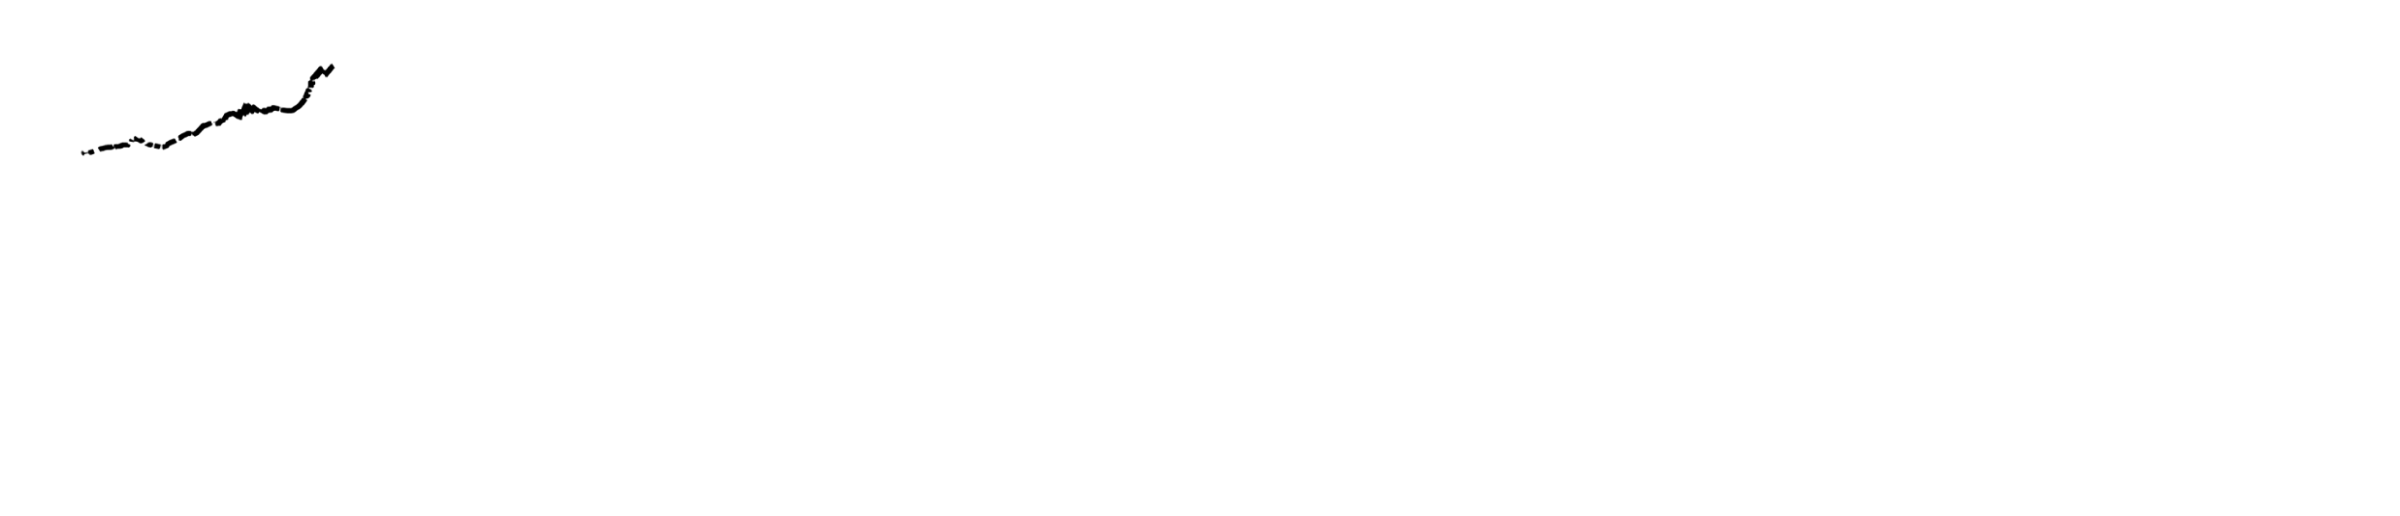
\includegraphics[width=\textwidth]{gen_stroke_samples_2}
         \caption{Start}
         \label{fig:training_strokes:a}
     \end{subfigure}
     \hfill
     \begin{subfigure}[b]{0.49\textwidth}
         \centering
         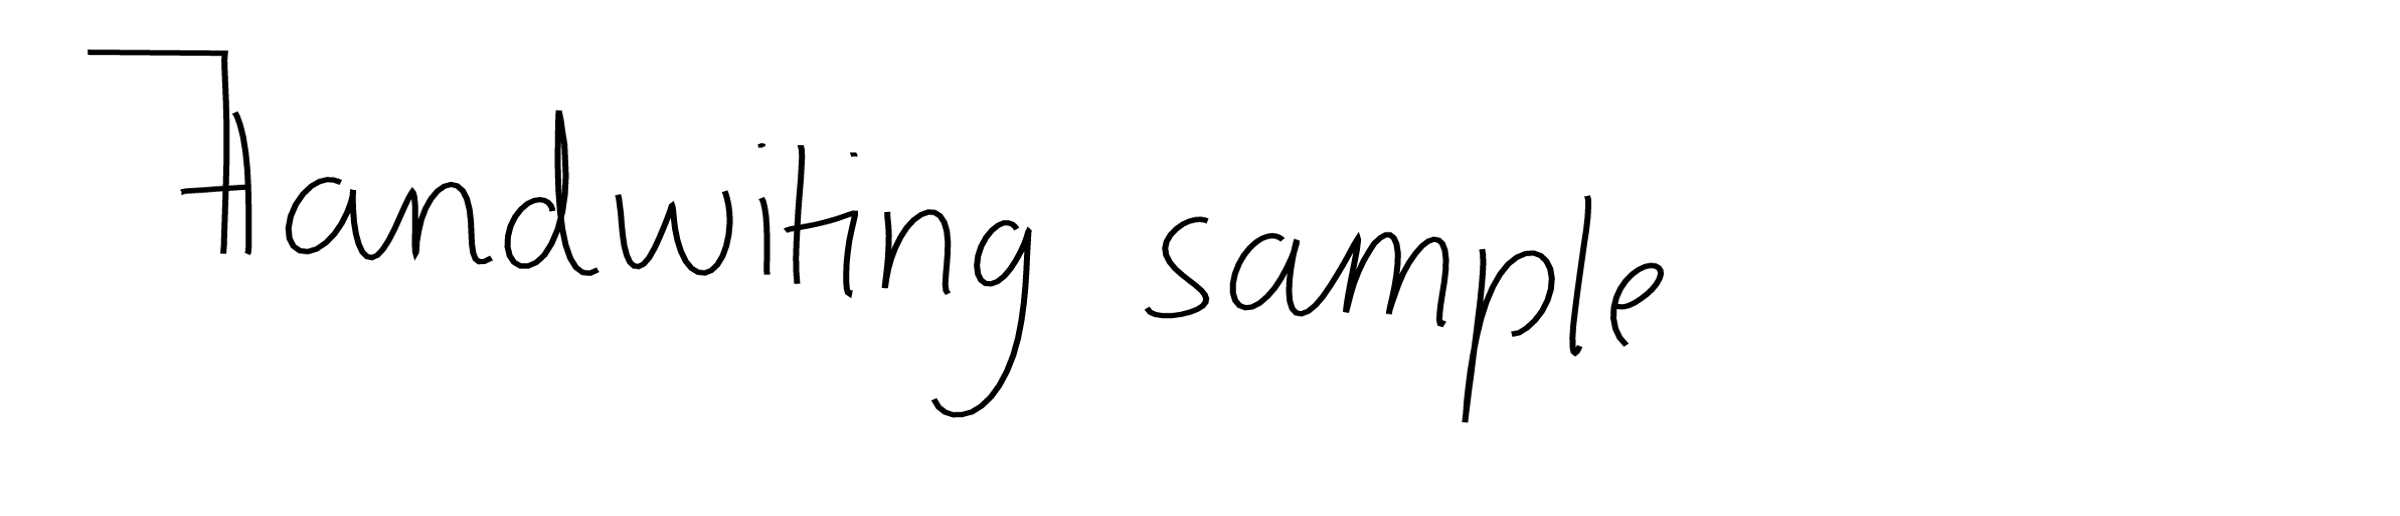
\includegraphics[width=\textwidth]{gen_stroke_samples_100}
         \caption{10 epochs}
         \label{fig:training_strokes:b}
     \end{subfigure}
     \newline
     
     \begin{subfigure}[b]{0.49\textwidth}
         \centering
         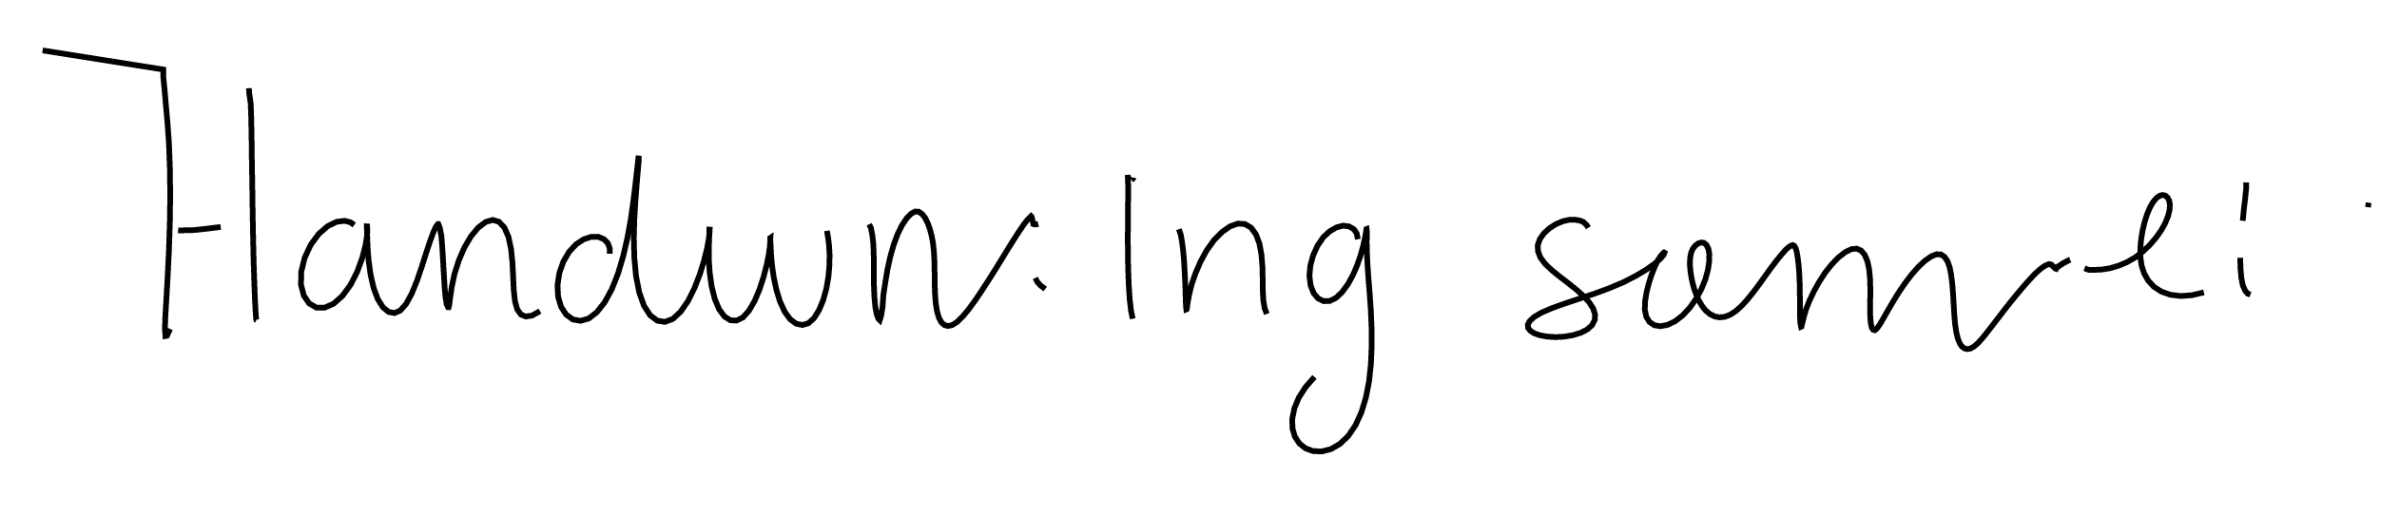
\includegraphics[width=\textwidth]{gen_stroke_samples_200}
         \caption{20 epochs}
         \label{fig:training_strokes:c}
     \end{subfigure}
     \hfill
     \begin{subfigure}[b]{0.49\textwidth}
         \centering
         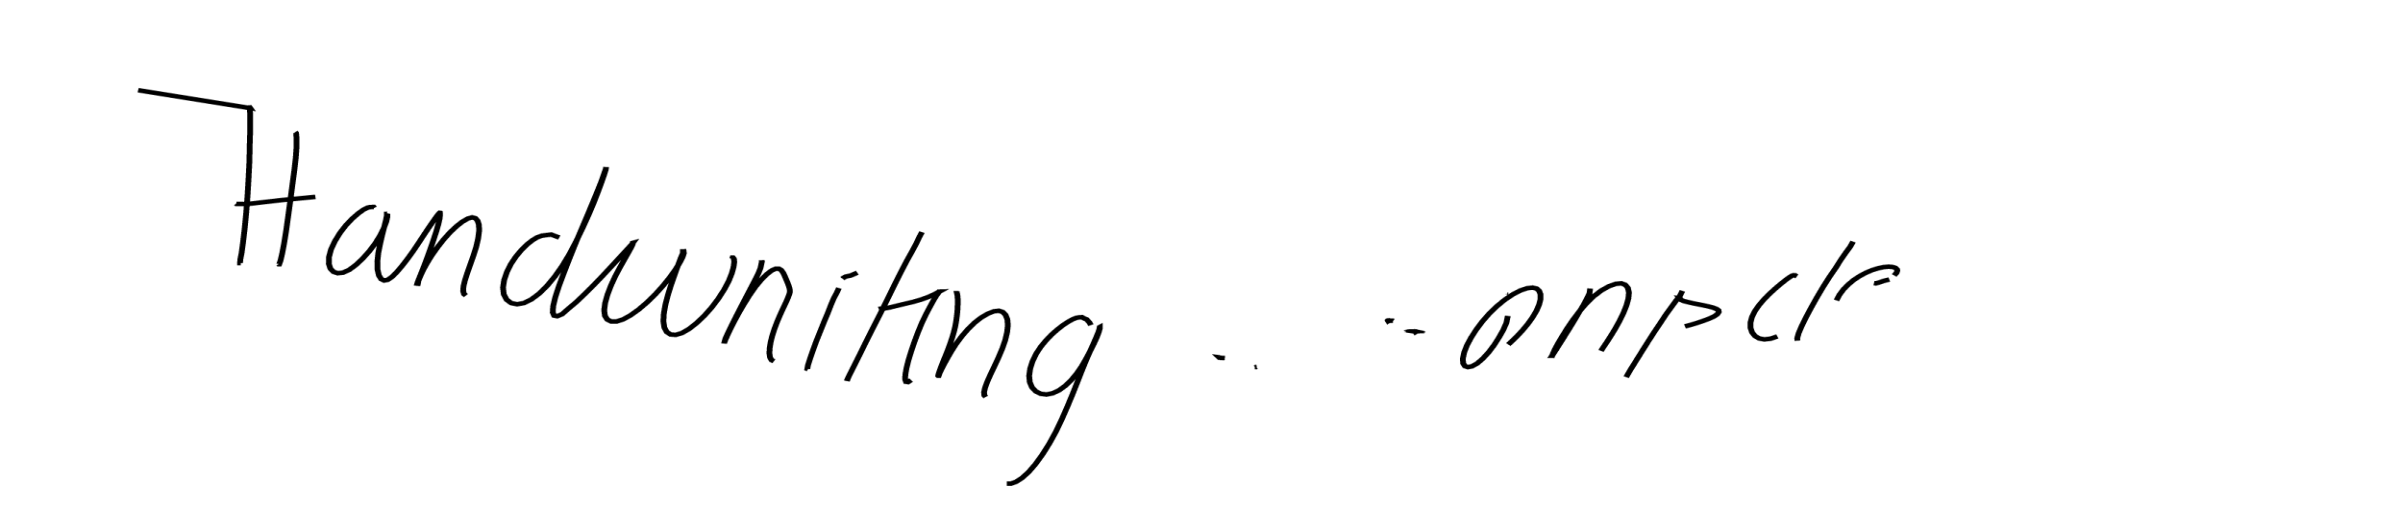
\includegraphics[width=\textwidth]{gen_stroke_samples_300}
         \caption{30 epochs}
         \label{fig:training_strokes:d}
     \end{subfigure}
     \newline
     
     \begin{subfigure}{0.49\textwidth}
         \centering
         
\includegraphics[width=\textwidth]{gen_stroke_samples_400}
         \caption{40 epochs}
         \label{fig:training_strokes:e}
     \end{subfigure}
     \hfill
     \begin{subfigure}{0.49\textwidth}
         \centering
         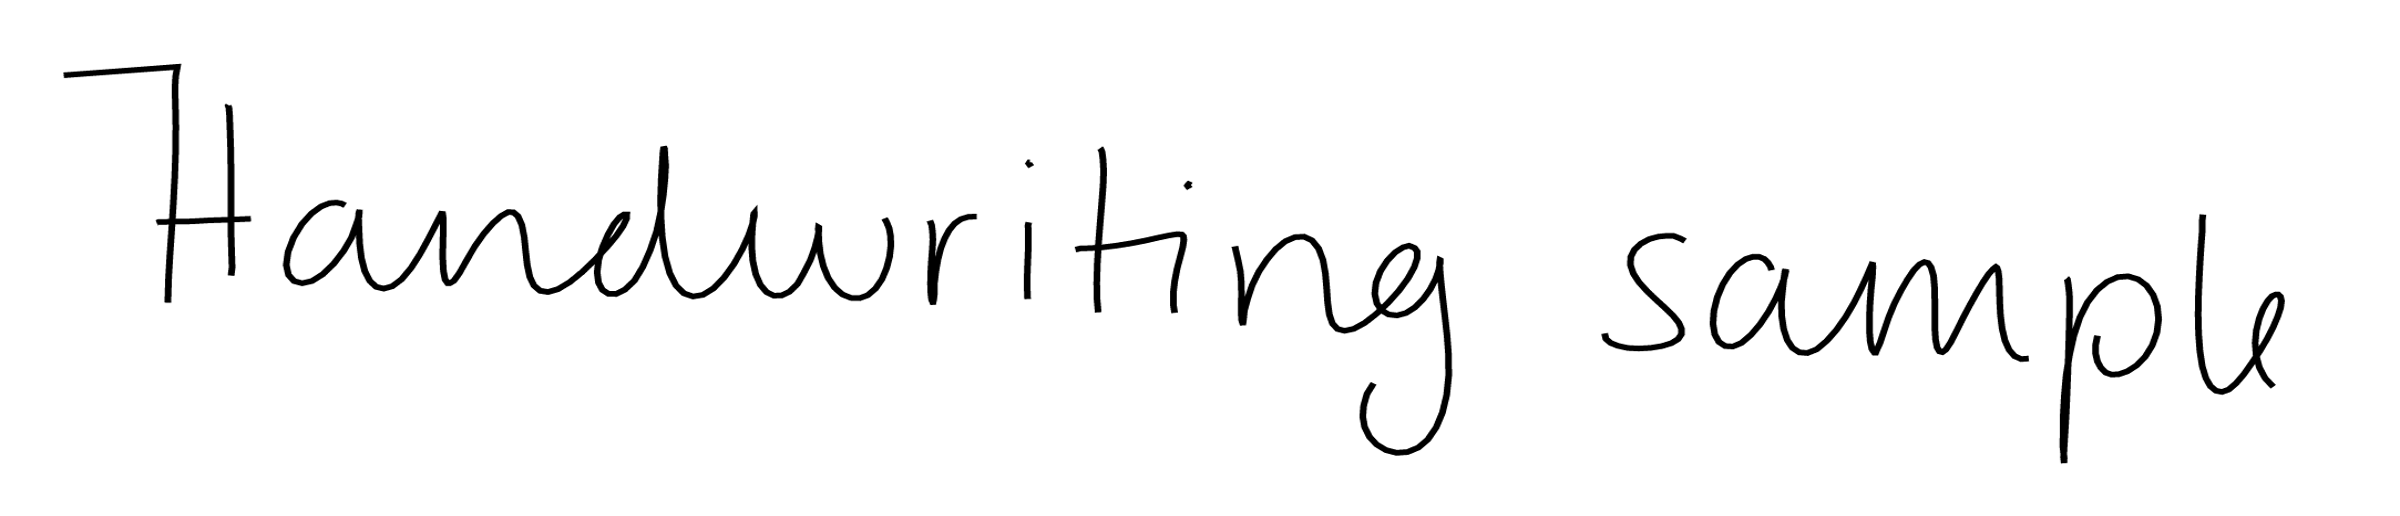
\includegraphics[width=\textwidth]{gen_stroke_samples_505}
         \caption{50 epochs}
         \label{fig:training_strokes:f}
     \end{subfigure}
     
    \caption{Stroke generation as training progresses}
    \label{fig:training_strokes}
\end{figure}

The second hook will save heat map plots of the training progress every 100 batches. These heat maps are illustrated in Figure ~\ref{fig:weight_heatmaps} and represent the training $\phi$s (more below) and soft attention windows at that point in the training. They are useful for understanding the math behind the training, for making sure training is proceeding as expected, and for selectively including in other publications like papers or reports.

\begin{figure}[hbt!]
     \centering
     \begin{subfigure}[b]{0.24\textwidth}
         \centering
         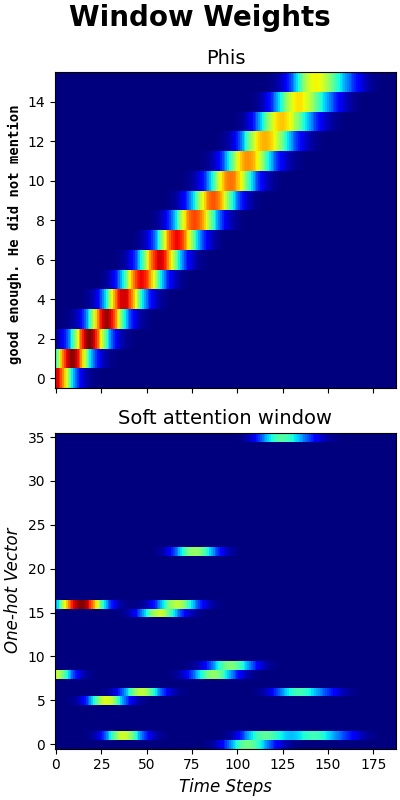
\includegraphics[width=\textwidth]{heatmap_weights_1}
         \caption{Start}
         \label{fig:weight_heatmaps:a}
     \end{subfigure}
     \hfill
     \begin{subfigure}[b]{0.24\textwidth}
         \centering
         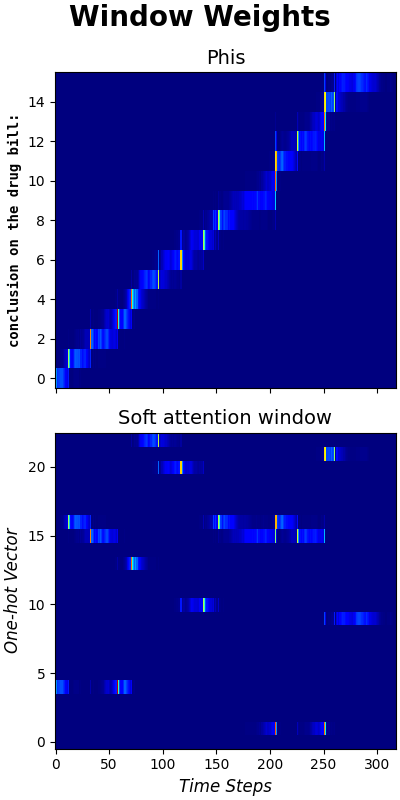
\includegraphics[width=\textwidth]{heatmap_weights_100}
         \caption{17 epochs}
         \label{fig:weight_heatmaps:b}
     \end{subfigure}
     \hfill
     \begin{subfigure}[b]{0.24\textwidth}
         \centering
         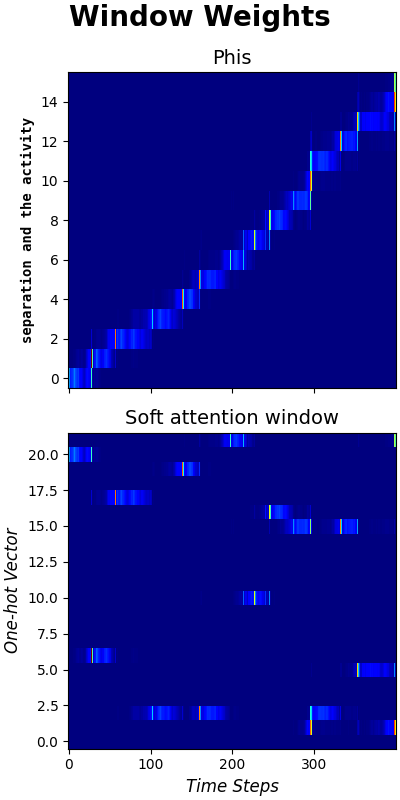
\includegraphics[width=\textwidth]{heatmap_weights_200}
         \caption{34 epochs}
         \label{fig:weight_heatmaps:c}
     \end{subfigure}
     \hfill
     \begin{subfigure}[b]{0.24\textwidth}
         \centering
         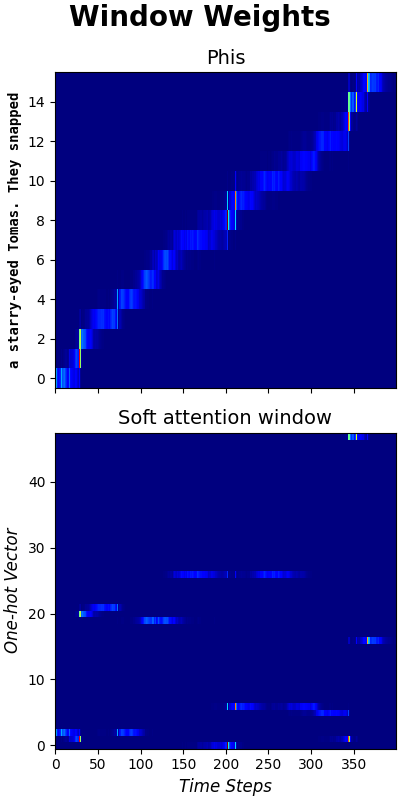
\includegraphics[width=\textwidth]{heatmap_weights_303}
         \caption{50 epochs}
         \label{fig:weight_heatmaps:d}
     \end{subfigure}

    \caption{Weight heat maps as training progresses}
    \label{fig:weight_heatmaps}
\end{figure}

The third hook, shown in figure ~\ref{fig:training_strokes}, generates a sample handwriting sequence every 500 batches. This is useful to see how the training is progressing and to understand what the model is doing at certain points in its execution.

Then, a fourth hook will trigger at the end of the training operation if the \textit{--test-model} flag is set. This will generate a final set of handwriting images in SVG format to validate the state of the trained model, as demonstrated in figure ~\ref{fig:hello}.

    \begin{figure}[hbt!]
        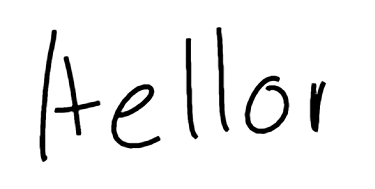
\includegraphics[width=6cm]{Sample}
        \centering
        \caption{Generated text: "\emph{Hello}"}
        \label{fig:hello}
    \end{figure}
    
\section{Results}
The training data set contained 12,195 handwriting samples.  Training took place on a university mainframe computer with GPU support.  Each epoch saw an improvement in the loss, with the largest (exponential) improvements recorded in the first 3 epochs.  After 50 epochs, the loss reached its minimum of -348.

    \begin{figure}[hbt!]
        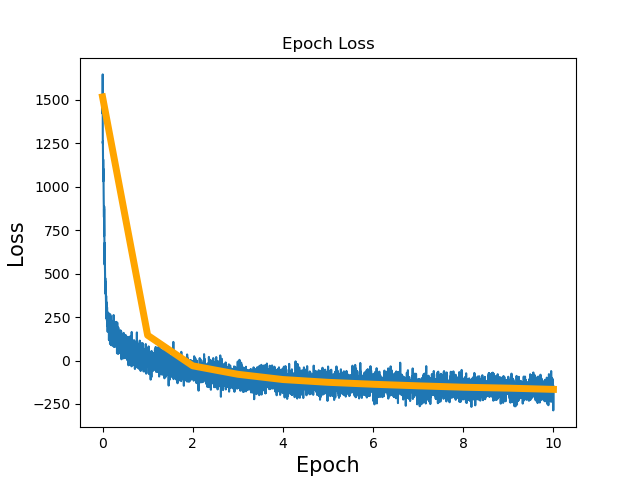
\includegraphics[width=12cm]{epoch_loss}
        \centering
        \caption{Epoch Loss}
        \label{fig:loss}
    \end{figure}
    
Handwriting generation resulted in the most realistic output as can be seen in Figure~\ref{fig:training_strokes:f} on page~\pageref{fig:training_strokes} and Figure~\ref{fig:hello} on page~\pageref{fig:hello}.

Smoothing results were less satisfactory than generation, as can be seen in Figure~\ref{fig:smoothed}.  In fact, results degraded as the bias values increased.  High biases were unrecognizable as handwriting, while lower biases were appeared worse than the original smoothing sample, which can be seen in Figure~\ref{fig:example_handwriting_line} on page~\pageref{fig:example_handwriting_line}.

    \begin{figure}[hbt!]
        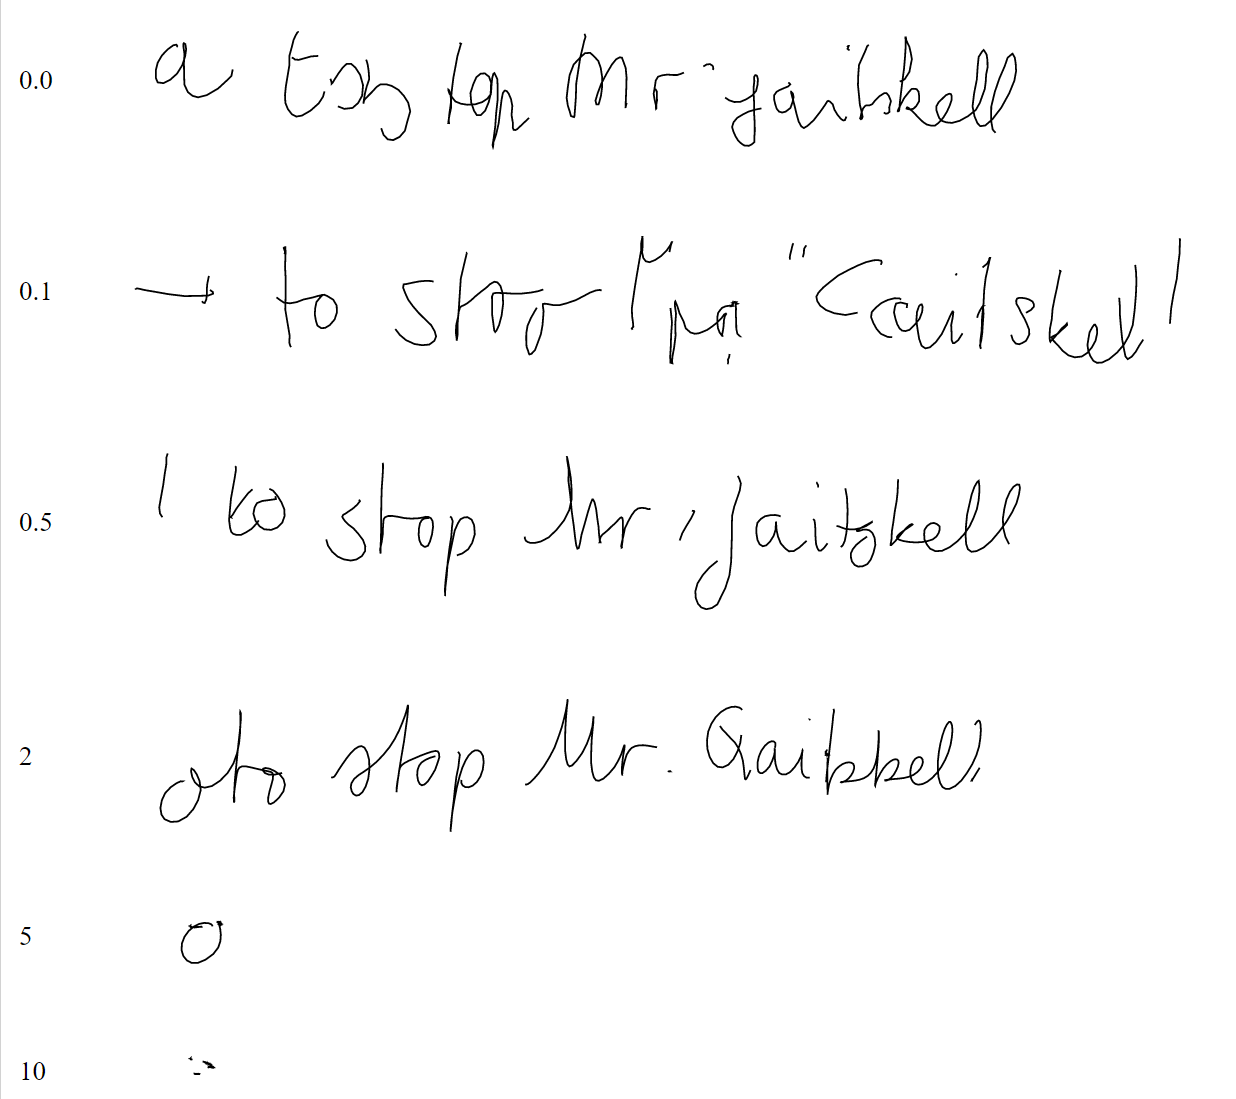
\includegraphics[width=12cm]{graphics/smooth_with_biases_1.png}
        \centering
        \caption{Smoothed handwriting sample with bias weights}
        \label{fig:smoothed}
    \end{figure}
    
Several approaches were tried to mitigate this effect, since Graves \cite{DBLP:journals/corr/Graves13} indicated that "priming" the network should  adjust the legibility via the biases while still retaining the handwriting style of the priming sample.  The one-hot vector was padded with spaces the length of the sample text, the original text was duplicated, and $\phi$ was pre-calculated from the sample sequence before feeding it into the trained network.  All approaches were unsuccessful, although (shown in Figure~\ref{fig:smoothed}) copying the original sample's sequence into the Pytorch tensor as the priming value before generating the smoothed sequence proved the most promising.
    
\section{Analysis}
An analysis of this project discusses how the LSTM network produces the handwriting results observed along with the role of statistical prediction and the structure of the loss function.

\subsection{Structure of the LSTM}
LSTM is short for \textit{Long Short-Term Memory}, meaning that the network has a built-in "memory". This is important for handwriting generation because future points along a stroke depend not just on the immediate predecessor to the stroke but also on several predecessors. For instance, to draw an \textit{S}, requires a series of points along the curve of the \textit{S}. It must differentiate between the curve of an \textit{S} as opposed to another character like a \textit{C} or even as opposed to a random sequence of points that makes no letter at all.

LSTM is a specialized form of an \textit{RNN} or \textit{Recurrent Neural Network} \cite{lstm-intro}. As such, any considerations for RNN will also apply to LSTM. RNNs in particular suffer from a phenomenon known as the vanishing gradient problem, and LSTMs address this. Gradients are those from mathematics, and they can "vanish" in a regular RNN because the network performs a multiplication at each iteration of training. Those stacked multiplications are the same, mathematically, as exponentiation, and exponentiation is an inherently unstable operation. Therefore, with each new multiplication the exponent grows. As the exponent grows very large, an operand less than one will grow very small and approach zero... thus, it "vanishes" over time. LSTMs solve this by replacing the multiplication with addition.

Though the original Graves paper \cite{DBLP:journals/corr/Graves13} is recommended reading for full understanding of LSTMs, here is a brief summary. 

The architecture of a regular RNN network looks like the figure below.

    \begin{figure}[hbt!]
        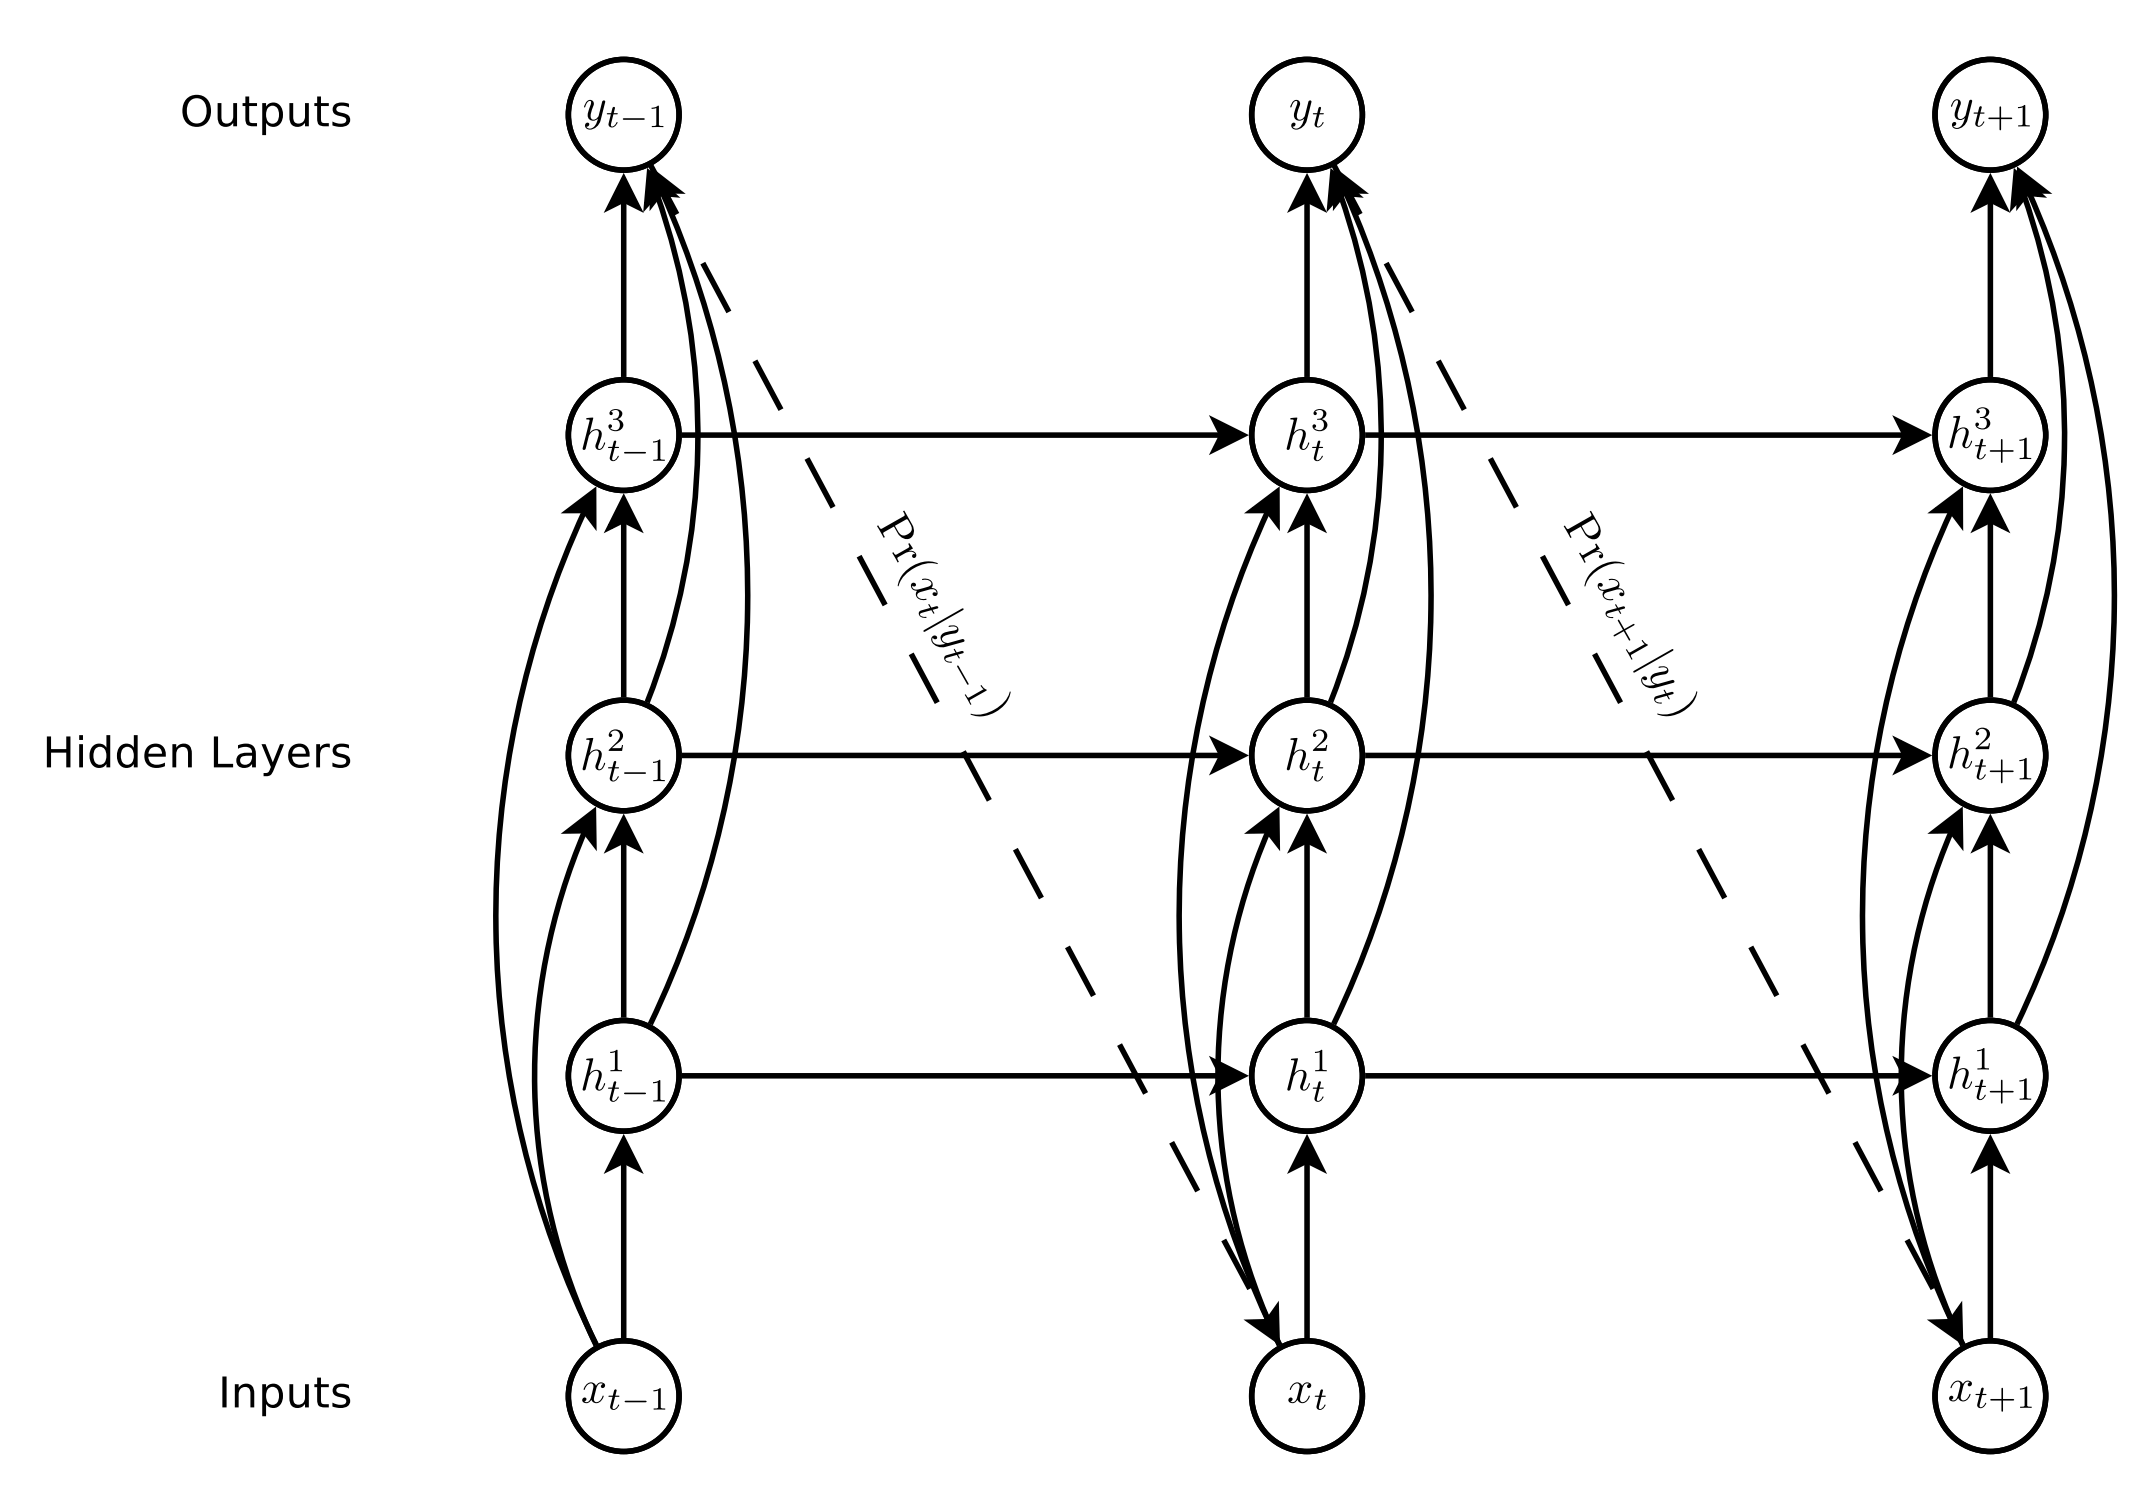
\includegraphics[width=12cm]{graphics/RNN-Arch.png}
        \centering
        \caption{Traditional recurrent neural network (RNN)}
        \label{fig:rnn}
    \end{figure}

As with any neural network, the design consists of an input layer, an output layer, and a series of hidden layers in between. The $x$ terms represent the location at points in time. Those pass through the hidden layers to the output layer. The output of a layer, which is a probability distribution of the next point, becomes the input to the next network iteration. So the output of $x_{n-1}$ becomes the input of $x_{n}$.

    \begin{align}
        \label{eqn:gr1} &h_t^1 = \mathcal{H}(W_{ih^1}x_t + W_{h^1h^1}h_{t-1}^1 + b_h^1) & \text{\tiny{(Graves\cite{DBLP:journals/corr/Graves13} eq. 1)}} \\
        \label{eqn:gr2} &h_t^n = \mathcal{H}(W_{ih^n}x_t + W_{h^{n-1}h^n}h_t^{n-1} + W_{h^nh^n}h_{t-1}^n + b_h^n) & \text{\tiny{(Graves\cite{DBLP:journals/corr/Graves13} eq. 2)}} 
    \end{align}

The hidden layer activations are calculated according to equations~\ref{eqn:gr1} (for the first hidden layer) and~\ref{eqn:gr2} (for the $n^{th}$ hidden layer) of the paper. The $W$ terms are weight matrices. In fact, most of the calculations will be done using linear algebra vectors and matrices for simplicity and performance. The output is computed according to equation~\ref{eqn:gr3} and~\ref{eqn:gr4}.

    \begin{align}
        \label{eqn:gr3} \hat{y_t} &= b_y + \sum_{n=1}^NW_{h^ny}h_t^n & \text{\tiny{(Graves\cite{DBLP:journals/corr/Graves13} eq. 3)}} \\
        \label{eqn:gr4} y_t &= \mathcal{Y}(\hat{y_t}) & \text{\tiny{(Graves\cite{DBLP:journals/corr/Graves13} eq. 4)}}
    \end{align}
    
At each iteration, a loss function is needed in order to determine how well the iteration did and to make adjustments. The loss function is given by equation~\ref{eqn:gr6}, which calculates partial derivatives and applies them via back-propagation to the network for use by the next iteration.

    \begin{equation}
        \label{eqn:gr6}  
        \mathcal{L}(x) = -\sum_{t=1}^T\log\text{Pr}(x_{t+1}\vert y_t) \quad\quad\quad \text{\tiny{(Graves\cite{DBLP:journals/corr/Graves13} eq. 6)}}
    \end{equation}

For an LSTM, a special cell is used for the hidden layer activation function, shown in Figure~\ref{fig:cell}. The cell is a group of equations that interact with each other to compute the final value of the hidden layer $h_{t}$. Then, that becomes $h_{t-1}$ when the cell is computed the next time through the network. Note that $i$, $f$, $o$, and $c$ correspond to each one of a function below, and $h$, also a function below, is computed from the others. These functions represent equations~\ref{eqn:gr7} -~\ref{eqn:gr11}.

    \begin{figure}[hbt!]
        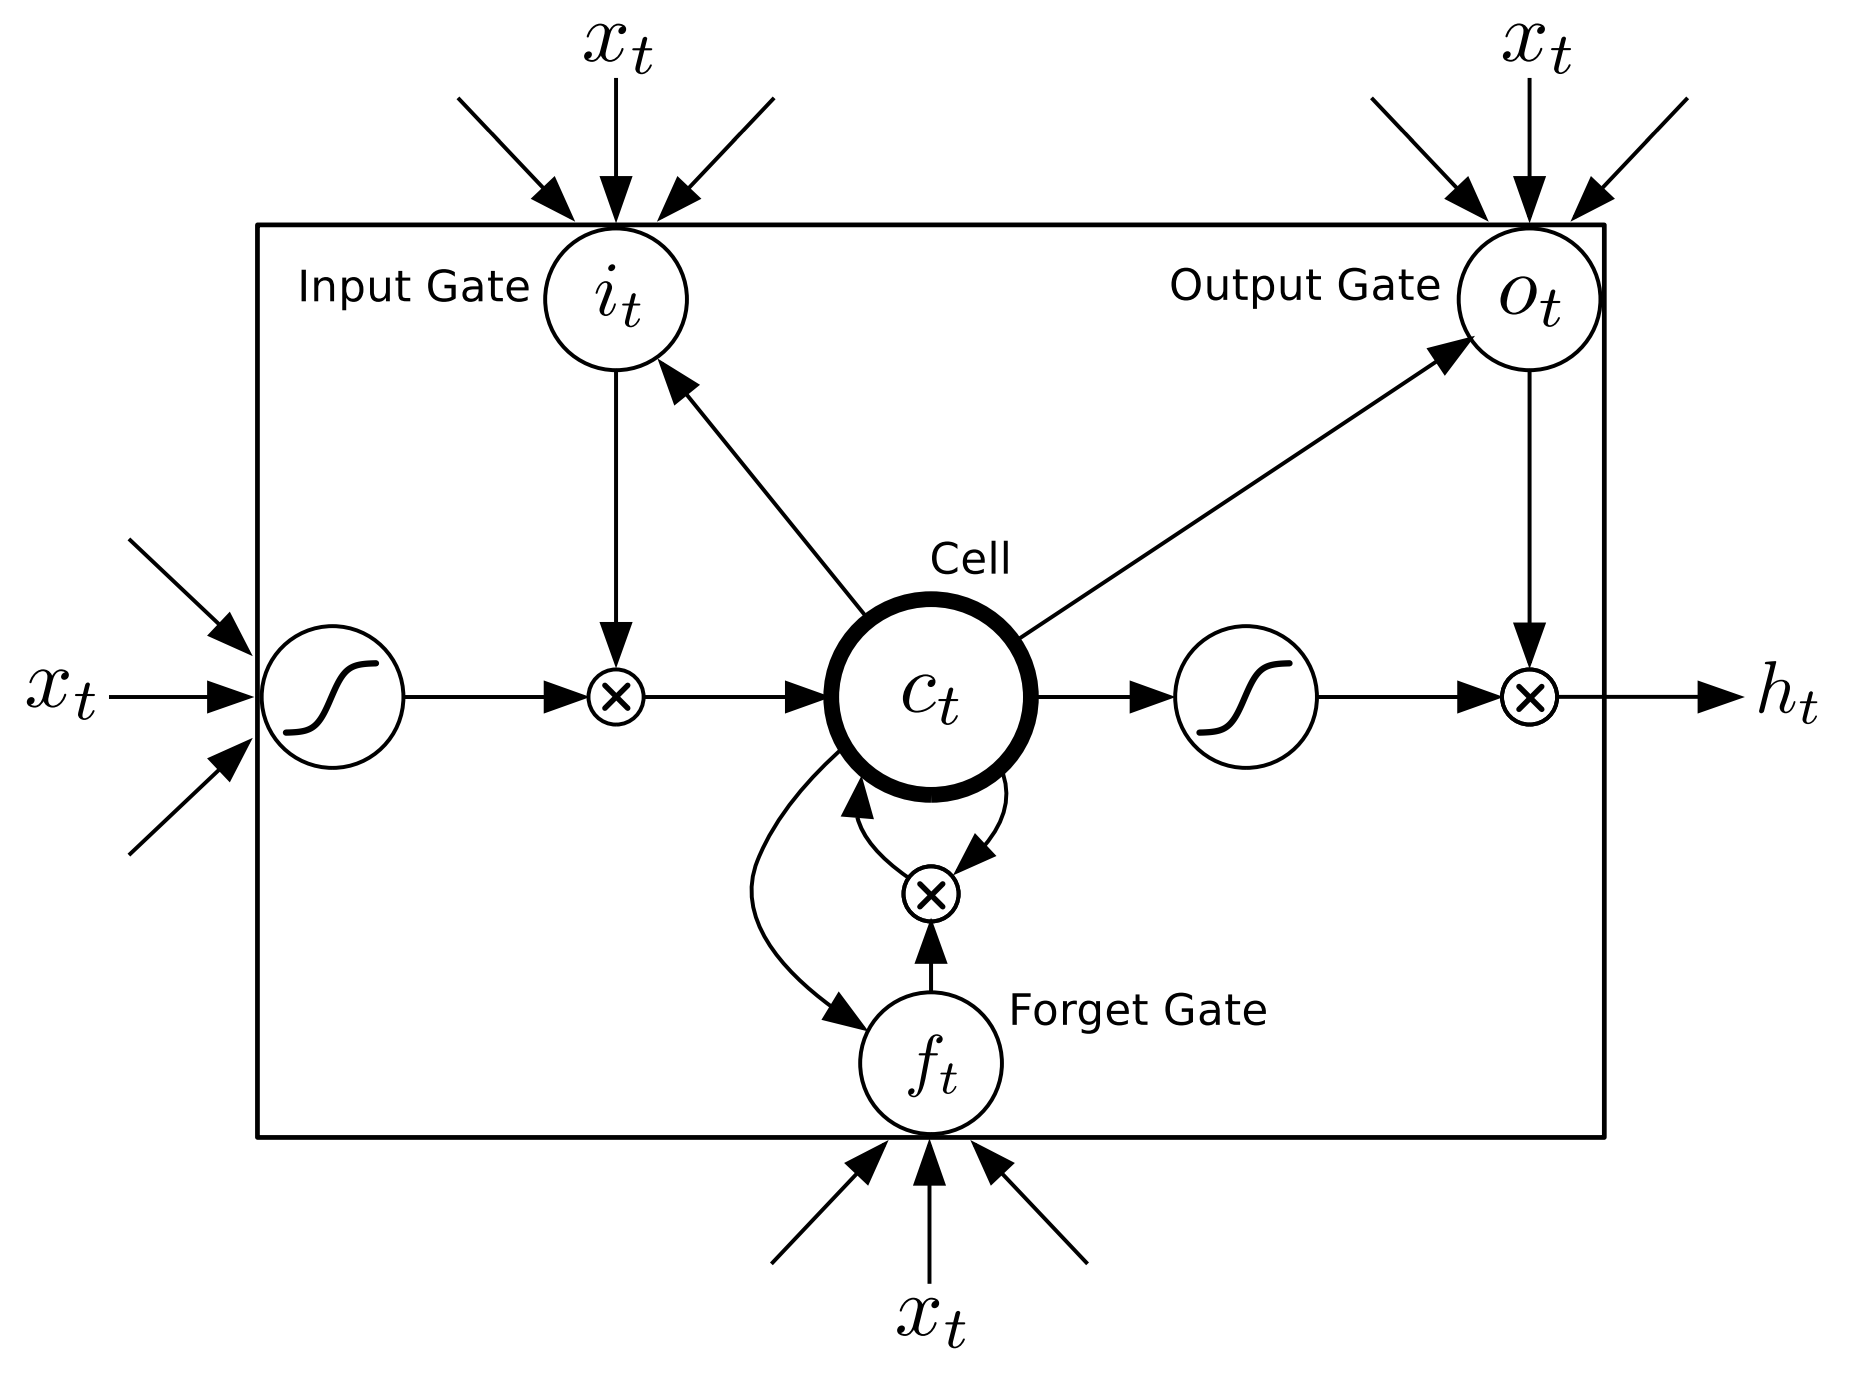
\includegraphics[width=12cm]{graphics/LSTM-Memory-Cell.png}
        \centering
        \caption{LSTM memory cell}
        \label{fig:cell}
    \end{figure}
    
    \begin{align}
        \label{eqn:gr7} i_t &= \sigma(W_{xi}x_t+W_{hi}h_{t-1}+W_{ci}c_{t-1}+b_i) & \text{\tiny{(Graves\cite{DBLP:journals/corr/Graves13} eq. 7)}} \\
        \label{eqn:gr8} f_t &= \sigma(W_{xf}x_t+W_{hf}h_{t-1}+W_{cf}c_{t-1}+b_f) & \text{\tiny{(Graves\cite{DBLP:journals/corr/Graves13} eq. 8)}} \\
        \label{eqn:gr9} c_t &= f_tc_{t-1}+i_t\tanh(W_{xc}x_t+W_{hc}h_{t-1}+b_c) & \text{\tiny{(Graves\cite{DBLP:journals/corr/Graves13} eq. 9)}} \\
        \label{eqn:gr10} o_t &= \sigma(W_{xo}x_t+W_{ho}h_{t-1}+W_{co}c_{t}+b_o & \text{\tiny{(Graves\cite{DBLP:journals/corr/Graves13} eq. 10)}} \\
        \label{eqn:gr11} h_t &= o_t\tanh(c_t) & \text{\tiny{(Graves\cite{DBLP:journals/corr/Graves13} eq. 11)}}
    \end{align}    
    
Using the longer (additive) memory in an LSTM instead of the shorter (multiplicative) memory of an RNN, has eliminated the vanishing gradient problem. However exploding gradients emerge, which is the opposite problem as before. Because of the unstable nature of exponentiation (the effect that comes into play over many iterations of the network training algorithm), the gradients (derivatives) computed at each iteration might expand to an exponentially large value. The solution is to "clip" the gradients so that they never exceed a certain value; in this project, they were clipped between -10 and 10.

To aid in understanding, Figure~\ref{fig:lstm} is another diagram of the same thing.
    
    \begin{figure}[hbt!]
        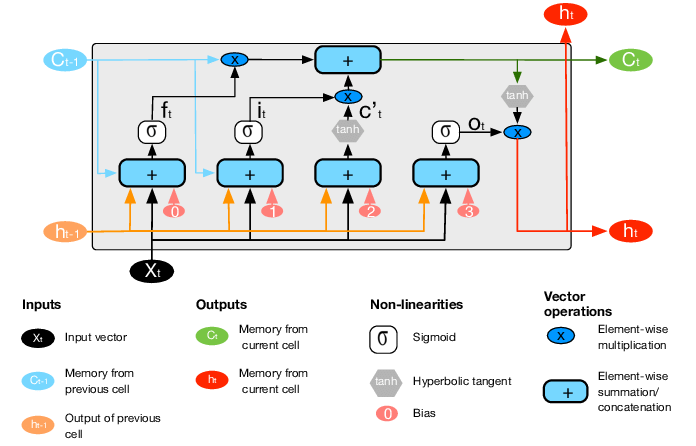
\includegraphics[width=12cm]{graphics/LSTM-Arch.png}
        \centering
        \caption{LSTM architecture \cite{inproceedings}}
        \label{fig:lstm}
    \end{figure}    
    
The same functions are noted in the earlier memory cell diagram and in the equations above: $i$, $f$, $o$, and $c$ along with the hidden output $h$. Code implemented from this will compute each piece using the inputs as shown on the diagrams/formulas. Then, those computed results will be used in subsequent computations as the calculation executes across the cell/layers. Outputs from one iteration become inputs to the next, and the process repeats for all of the inputs in the current batch, then across all the batches in the epoch, then for each of the epoch in the training.

\subsection{Mixture Densities}
This is a key part of handwriting generation. The network computes a statistical probability function that represents the odds that the next point in the stroke will be at a certain position. The distribution is normalized, which makes it easy to differentiate. For example, in drawing an \textit{S}, the current point is at the end of the series of connected points along the x/y axis. It is expected that the next likely point will be somewhere in an oval space around the current point. Because it is an \textit{S}, the distribution would be skewed a bit to the next part of the \textit{S} stroke (because the network was trained, it knows how to draw an \textit{S}). Figure~\ref{fig:bivariate} shows a visual diagram of what is going on here (minus the \textit{S} strokes).
    
    \begin{figure}[hbt!]
        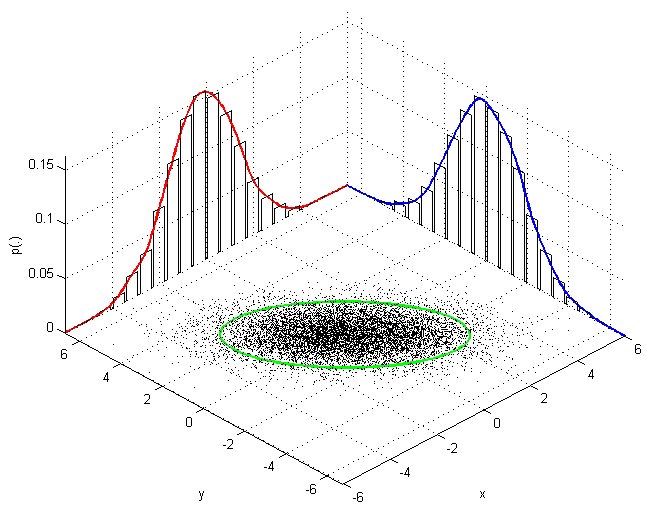
\includegraphics[width=12cm]{graphics/Bivariate-example.png}
        \centering
        \caption{Bi-variate example \cite{monteiro}}
        \label{fig:bivariate}
    \end{figure}    
    
The oval represents the possible points, but notice that the oval is composed of two (i.e. the "bi" in bi-variate) histograms, which are just the probabilities of $x$ and of $y$. The Gaussian mixture is expressed by equations 23 - 25 in the Graves paper \cite{DBLP:journals/corr/Graves13}.

    \begin{align}
        \label{eqn:gr23} &\text{Pr}(x_{t+1}\vert y_t) = \sum_{j=1}^M\pi_t^j\mathcal{N}(x_{t+1}\vert\mu_t^j,\sigma_t^j,\rho_t^j)
        \begin{cases}
            e_t,& \text{if } (x_{t+1})_3=1\\
            1 - e_t,& \text{otherwise}
        \end{cases} &
        \text{\tiny{(Graves\cite{DBLP:journals/corr/Graves13} eq. 23)}} \\
        \label{eqn:gr24} &\mathcal{N}(x\vert\mu,\sigma,\rho) = \frac{1}{2\pi\sigma_1\sigma_2\sqrt{1-\rho^2}}\exp\left[\frac{-Z}{2(1-\rho^2)}\right] & \text{\tiny{(Graves\cite{DBLP:journals/corr/Graves13} eq. 24)}} \\
        \label{eqn:gr25} &Z = \frac{(x_1-\mu_1)^2}{\sigma_1^2} + \frac{(x_2 - \mu_2)^2}{\sigma_2^2} - \frac{2\rho(x_1-\mu_1)(x_2-\mu_2)}{\sigma_1\sigma_2} & \text{\tiny{(Graves\cite{DBLP:journals/corr/Graves13} eq. 25)}}
    \end{align}

The paper \cite{DBLP:journals/corr/Graves13} also goes through the derivation of the loss function, which is in turn used to update the weights of the network in back-propagation, as usual. The most likely point is then chosen from the distribution and used as the starting point of the next iteration. The end point, which is the point at which the pen is lifted, is also computed, and this is how the network knows when to end one stroke and begin the next.

\subsection{Handwriting Synthesis Model}
The key method of the model implementation is \textit{forward()}, which will be called repeatedly by the trainer. This method represents the forward propagation. It takes $x$ and $c$ as inputs.

$x$ is a batch of stroke coordinates of sequences. Its dimensions are [sequence\_size, batch\_size, 3]. The 3 corresponds to $x$ and $y$ offset of a stroke and \textit{eos} [which equals 1 when reaching an end of stroke (when the pen is raised)].

$c$, a batch of one-hot encoded sentences corresponding to the stroke sequence is of dimensions [n\_batch, U\_items, len(alphabet)]. Note that the forward function is also used to generate random sequences.

The first step is to compute LSTM1. This is straightforward in PyTorch. Since the LSTM cells use Pytorch, we need a \textit{for} loop over the whole stroke sequence.

After LSTM1, the code computes the attention mechanism given by equations~\ref{eqn:gr46} -~\ref{eqn:gr51}.

    \begin{align}
        \label{eqn:gr46} \phi(t,u) &= \sum_{k=1}^K\alpha_t^kexp[-\beta_t^k(\kappa_t^k-u)^2] & \text{\tiny{(Graves\cite{DBLP:journals/corr/Graves13} eq. 46)}} \\
        \label{eqn:gr47} w_t &= \sum_{u=1}^U\phi(t,u)c_u & \text{\tiny{(Graves\cite{DBLP:journals/corr/Graves13} eq. 47)}} \\
        \label{eqn:gr48} (\hat{\alpha}_t,\hat{\beta}_t,\hat{\kappa}_t) &= W_{h^1p}h_t^1 + b_p & \text{\tiny{(Graves\cite{DBLP:journals/corr/Graves13} eq. 48)}} \\
        \label{eqn:gr49} \alpha_t &= exp(\hat{\alpha}_t) & \text{\tiny{(Graves\cite{DBLP:journals/corr/Graves13} eq. 49)}} \\
        \label{eqn:gr50} \beta_t &= exp(\hat{\beta}_t) & \text{\tiny{(Graves\cite{DBLP:journals/corr/Graves13} eq. 50)}} \\
        \label{eqn:gr51} \kappa_t &= \kappa_{t-1} + exp(\hat{\kappa}_t) & \text{\tiny{(Graves\cite{DBLP:journals/corr/Graves13} eq. 51)}}
    \end{align}  
    
After that, the network computes LSTM2 and LSTM3. Then it is just a matter of computing equations~\ref{eqn:gr18} -~\ref{eqn:gr22} using a dense layer.

    \begin{align}
        \label{eqn:gr18} e_t = \frac{1}{1+exp(\hat{e}_t)} & \Longrightarrow e_t\in(0,1) & \text{\tiny{(Graves\cite{DBLP:journals/corr/Graves13} eq. 18)}} \\
        \label{eqn:gr19} \pi_t^j = \frac{exp(\hat{\pi}_t^j)}{\sum_{j'=1}^Mexp(\hat{\pi}_t^{j'})} & \Longrightarrow \pi_t^j\in(0,1), \sum_{j}\pi_t^j=1 & \text{\tiny{(Graves\cite{DBLP:journals/corr/Graves13} eq. 19)}} \\
        \label{eqn:gr20} \mu_t^j = \hat{\mu}_t^j & \Longrightarrow \mu_t^j\in\mathbb{R} & \text{\tiny{(Graves\cite{DBLP:journals/corr/Graves13} eq. 20)}} \\
        \label{eqn:gr21} \sigma_t^j = exp(\hat{\sigma}_t^j) & \Longrightarrow \sigma_t^j>0 & \text{\tiny{(Graves\cite{DBLP:journals/corr/Graves13} eq. 21)}} \\
        \label{eqn:gr22} \rho_t^j = \tanh(\hat{\rho}_t^j) & \Longrightarrow \rho_t^j\in(-1,1) & \text{\tiny{(Graves\cite{DBLP:journals/corr/Graves13} eq. 22)}}
    \end{align}  
    
The algorithm will continue until it reaches the stopping condition.  Since strokes will nearly always take a variable number of points to construct, it is not a simple matter of enumerating through a \textit{for} loop. Instead, the algorithm must compare the computed $\phi$ to the collection of previous $\phi$s. When the computed $\phi$ becomes greater than any prior value, then the algorithm has reached the end of the sequence and can stop.

\subsection{Loss Function}
First, the same configuration is used as in the Graves paper \cite{DBLP:journals/corr/Graves13}. The input layer is size 3, and there are 3 hidden layers with 400 cells in each one. The output layer has 20 bi-variate Gaussian mixture components. The loss function uses stochastic gradient descent. Once trained, the same configuration is used to generate or smooth handwriting.

Going back to the implementation of \textit{LSTMTrainer}, the \textit{train\_network()} method first calls the \textit{forward()} method of the \textit{HandwritingSynthesisModel}, which is a standard method implemented as specified by Pytorch. This method automatically computes the gradient weight updates to the network.

The \textit{forward()} gives the values needed in order to compute the Gaussian mixture (eqs.~\ref{eqn:gr23} -~\ref{eqn:gr25}), namely $y$, $\pi$, $\mu_1$, $\mu_2$, $\sigma_1$, $\sigma_2$ and $\rho$. These become the input to the \textit{gaussian\_mixture()} method, which returns the computed probability of the next $x$ given $y$.

Finally, the algorithm compares the predicted value to the actual value from the training data using the \textit{loss\_fn()}. The result is used to propagate backward through the network and update the weights. The gradients are also clipped as described above at this point. After every epoch, the state of the model is saved so it can be reloaded later to save time.

\subsection{Generating Handwriting}
The next step is to generate sequences of stroke points that will form the generated sample. In order to generate a handwriting sample, a slight modification is made to the network architecture that is shown in Figure~\ref{fig:cell-with-c}, to add a character $c$ input.  The character $c$ is specified prior to the input layer. This character is then inserted in between the hidden layers as a one-hot-encoded vector. The computation of the network then proceeds as normal. As described previously, the window weights $\phi$ are examined to determine the stopping condition: $\phi(t,U+1) > \phi(t,u) \quad \forall \quad 1\leq u\leq U$

The resulting style is consistent within itself but distinct from other sequences. A generated sequence will have the same handwriting style for the entire sequence. However, generating the sequence again, with the same or different character input, will result in a different handwriting style.

In the code, the method \textit{as\_handwriting()} is used to generate the handwriting sequence and to optionally display/save it according to the options that have been set.

\subsection{Smoothing Handwriting}
Smoothing is very similar to generation; however, instead of relying on a text string, the generator takes a sample of existing handwriting. The sample is input to the generation sequence to \textit{prime} the sequence. This gives the LSTM network a history of data points from which it will predict the next set of points. That lets it maintain the same style as the source handwriting.

To improve the handwriting, a bias term a bias term $b$ is added to the Gaussian mixture equations, as shown in equations~\ref{eqn:gr61} -~\ref{eqn:gr62}. This reduces the variation in point prediction and maintains the style.

    \begin{align}
        \label{eqn:gr61} \sigma_t^j &= exp(\hat{\sigma}_t^j-b) & \text{\tiny{(Graves\cite{DBLP:journals/corr/Graves13} eq. 61)}} \\
        \label{eqn:gr62} \pi_t^j &= \frac{exp\left(\hat{\pi}_t^j(1+b)\right)}{\sum_{j'=1}^Mexp\left(\hat{\pi}_t^j(1+b)\right)} & \text{\tiny{(Graves\cite{DBLP:journals/corr/Graves13} eq. 62)}}
    \end{align}  
    
Lower biases have less effect on the stylistic improvement, whereas higher biases result in cleaner handwriting at a cost of reduced stylistic distinctness. Values closer to 0 had the least effect and closer to 10 had the greatest effect.

In the code, the method \textit{smooth\_handwriting()} is used to smooth the supplied handwriting sequence and to optionally display/save it according to the options that have been set. The sequence is provided in a data file of the same format online format as the training data set. Internally, the sample is simply an instantiation of the \textit{Dataset} class described previously.

    
\section{Discussion}    
Compared to other learning disabilities, the symptoms of Dysgraphia may appear mild; however, it poses a significant life-long challenge \cite{previous-work-29}. This project establishes an application with an extendable frame work, published on GitHub. The application plots handwriting on a Cartesian grid, and then smooths the writing into a legible style similar to the original.

The application can be integrated into any device that is capable of running Python scripts. Potential field applications include: note taking for school and home, auto-filling forms with the person's writing style, and Dysgraphia diagnostic tools. Diagnostic tools could help to identify early childhood neural disorder and provide help during preschool years\cite{previous-work-31}.

Determining which neural networks method are best suited for handwriting smoothing was difficult. The initial thought was focusing on image (offline) processing based methods like GAN and Style Transfer\cite{previous-work-26}, this is the area where the majority of previous work was completed,including the transcription of old cursive historian records. A significant amount of time was spent on various image processing models. Dysgraphia handwriting posed a higher level of difficulty due to the significant slants, as well as uneven spacing and amplitude. Image processing relies on fairly reasonable spacing to recognize the end of a word and on comparable amplitude for pixel by pixel processing. The results were mixed and inconsistent for image based model.The pen stroke position (online) based LSTM model resulted in useful and the most promising models. 

\section{Future Work}
In the course of exploring techniques for this project, a lot of information was gathered about \textit{GAN}s, or \textit{Generative Adversarial Networks}. It would be interesting to explore using \textit{GAN}s to replicate the generative and smoothing work presented here. Such a network could be utilized to convert handwriting from an image into the online $x$, $y$ format needed for smoothing. It would also be interesting to find a way to minimize stylistic variance when using the bias adjustment technique while still improving the legibility.

An obvious next step would be to iron out the difficulties this project faced with priming the handwriting sequence in order to smooth out handwriting.  In fact, that would likely yield positive results quickly since the original paper \cite{DBLP:journals/corr/Graves13} was able to get it to work.  Thus, it would simply be a matter of replicating that success in the Python framework.

\section{Ethical Implications}
Overall, the ethical implications of handwriting recognition and smoothing are positive. The techniques shown in this paper could be applied in helping children and adults with Dysgraphia, as well as other disorders that affect handwriting like Parkinson's disease or arthritis. This work could also be used in the recreation of important archaic documents or transcripts that, with time, have become illegible.

Although the negative ethical implications are few, there is the potential for forgery which could lead to theft, misrepresentation, or mischief. With any new technology, security measures could be implemented to prevent such cases.

\section{Conclusion}
Dysgraphia is a disorder that affects the fine motor skills of both children and adults. This project explored possible ways of using neural networks to help people suffering from this disorder smooth out their hand writing to help them to better communicate. The end product of this project is an application that takes handwriting data, in the form of a sequential stroke data, as an input and generates a set of stroke data that would represent new smooth handwriting. The application can also take in training data sets that can be used to train a new model. This application will not only help people with Dysgraphia, but could promote additional research in many other areas of handwriting or hand drawing applications.

\medskip

\bibliography{dysgraphia}

\appendix
\section{Appendix}

\end{document}